\documentclass[10pt]{article}

% File icdp2009.sty
% Preamble that you have to include to use the template  

% July 24, 2009
% Contact: simonnet@ecole.ensicaen.fr


\usepackage[a4paper,textwidth=18cm,textheight=24cm,top=2.85cm, bottom=2.85cm, left=1.5cm, right=1.5cm]{geometry}

\usepackage{../template/icdp2009}

% left justified caption
\makeatletter
\long\def\@makecaption#1#2{%
\vskip\abovecaptionskip
\sbox\@tempboxa{#1. #2}%
\ifdim \wd\@tempboxa >\hsize
#1. #2\par
\else
\global \@minipagefalse
\hb@xt@\hsize{\box\@tempboxa\hfil}%
\fi
\vskip\belowcaptionskip}
\makeatother




%other package

% vectorial font
\usepackage{lmodern}

\usepackage{graphicx}
\usepackage{times}
\usepackage{booktabs}
\usepackage{siunitx}
\usepackage{adjustbox}
\usepackage{multirow}


\begin{document}
\noindent

% This should produce references in the order they appear
\bibliographystyle{ieeetr}

\title{Optical Waveguides: Theory and Implementation}

\authorname{Anirudh Prakash, Grace Liu, Surya Chandramouleeswaran}
\authoraddr{\textbf{\emph{A special thanks to Professor Maysam Chamanzar}}}



\maketitle


\abstract
Replace this with a succint summary of our work. Aim for 100 words  

\section{Introductory Concepts}
Discuss introductory concepts here, something like motivations works well too

\subsection{Understanding a particular concept}
Use subsections to illustrate subconcepts like this
\begin{figure}[h]
    \centering
    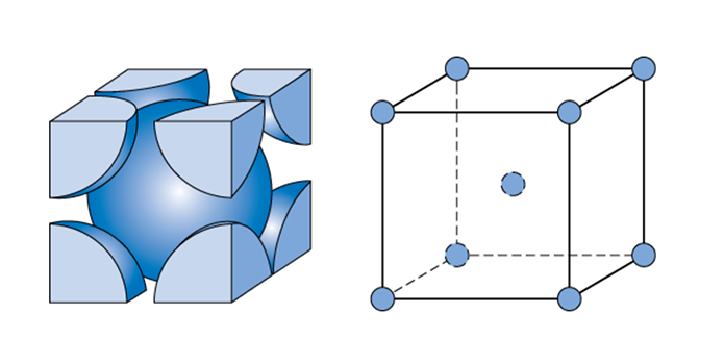
\includegraphics[width=8.5cm]{fig1}
    \caption{\label{tab1} Sample syntax for image, caption and citation. Adapted from \cite{ref01}.} 
    \end{figure}

When the steel is heated upto very high temperatures, the BCC ferrite phase transforms into the austenite phase, occupying a Face-Centered-Cubic (FCC) unit cell structure as seen in \textbf{Figure 2}.
\begin{figure}[h]
    \centering
    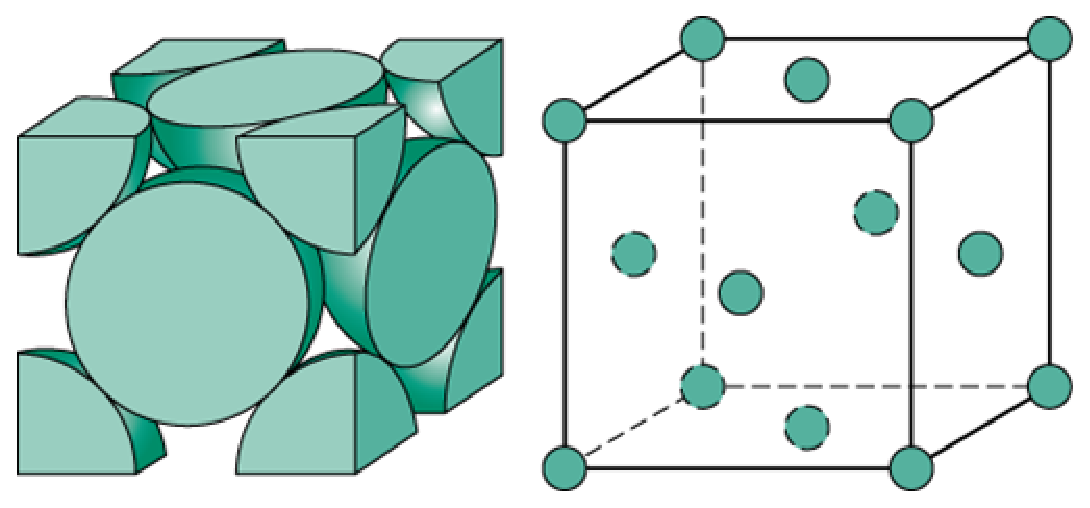
\includegraphics[width=8.5cm]{fig2}
    \caption{\label{tab1}FCC Unit Cell structure, with atoms at each of the faces of the cell cube. Adapted from \cite{ref01}.} 
    \end{figure}

\begin{figure}[h]
    \centering
    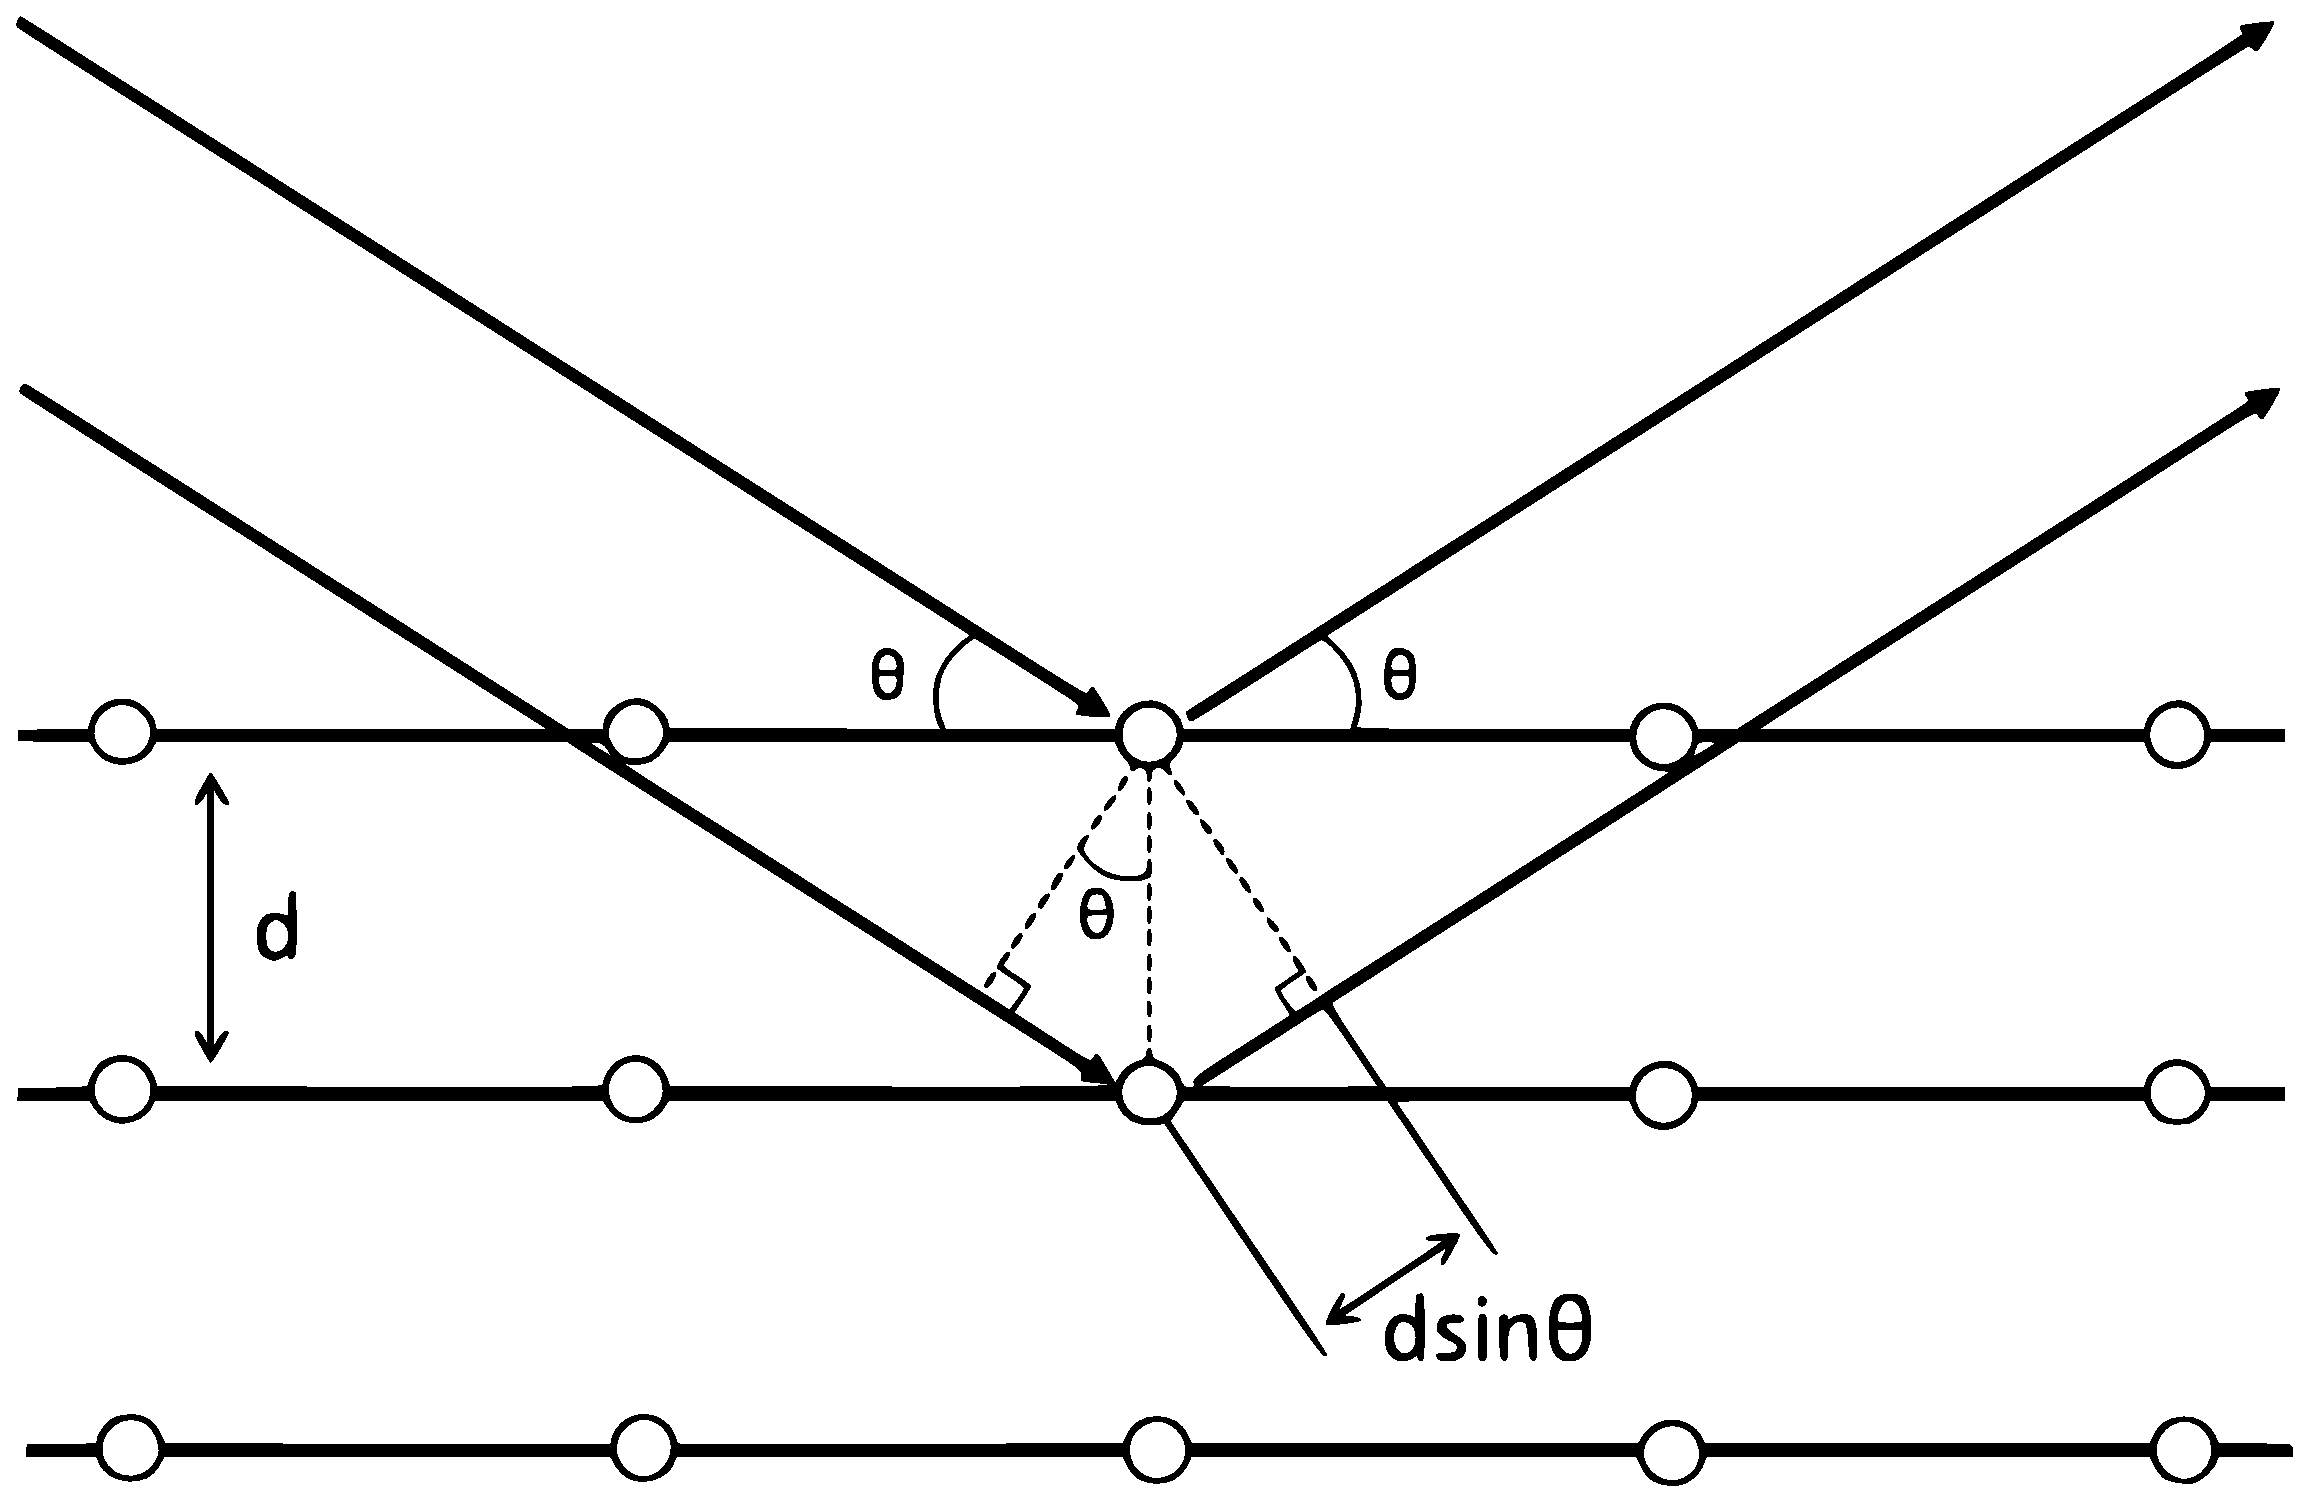
\includegraphics[width=8.5cm]{fig3}
    \caption{\label{tab1}An illustrative example of X-ray diffraction at the atomic level. Waves are represented by red arrows,
    $d$ stands for atomic spacing, and $\theta$ stands for the angle at which the X-ray beam enters the crystal lattice. File is licensed with CC BY 3.0. To view a copy of this license, 
    visit https://creativecommons.org/licenses/by/3.0.} 
    \end{figure}

After experiencing diffraction due to the interatomic spacings, the X-ray beams travel upwards towards a "detector," 
which measures the magnitude of X-ray beams that collide with its screen (this magnitude is represented by the unit \textbf{intensity}). Because of the repeating and symmetric 
arrangement of atoms in any given grain, multiple X-ray beams can experience diffraction phenomena and interfere with each other before being measured by the detector \cite{ref03}. 
X-ray beams can either \textit{constructively} interfere (such that the amplitude of the resulting wave comprises the sum of each individual 
wave amplitudes), or \textit{destructively} interfere (such that the amplitude of the ensuing wave cancels out due to the individual waves being out of phase with each other). 
Constructive interference of X-ray beams will lead to very high intensity readings by the XRD machine, while destructive interference of X-ray beams will not 
be registered by the detector, leading to no intensity readings by the XRD machine.

The machine used to conduct XRD experiments are called \textbf{X-ray Diffractometers}, which are made up of an X-ray source which varies the angle of X-ray beam impact onto the sample, a cradle to
stabilize and rotate (if need be) the sample, and a detector (mentioned above) which records the necessary measurements. A labeled figure of the X-ray diffractometer is shown in \textbf{Figure 4}.
\begin{figure}[h]
    \centering
    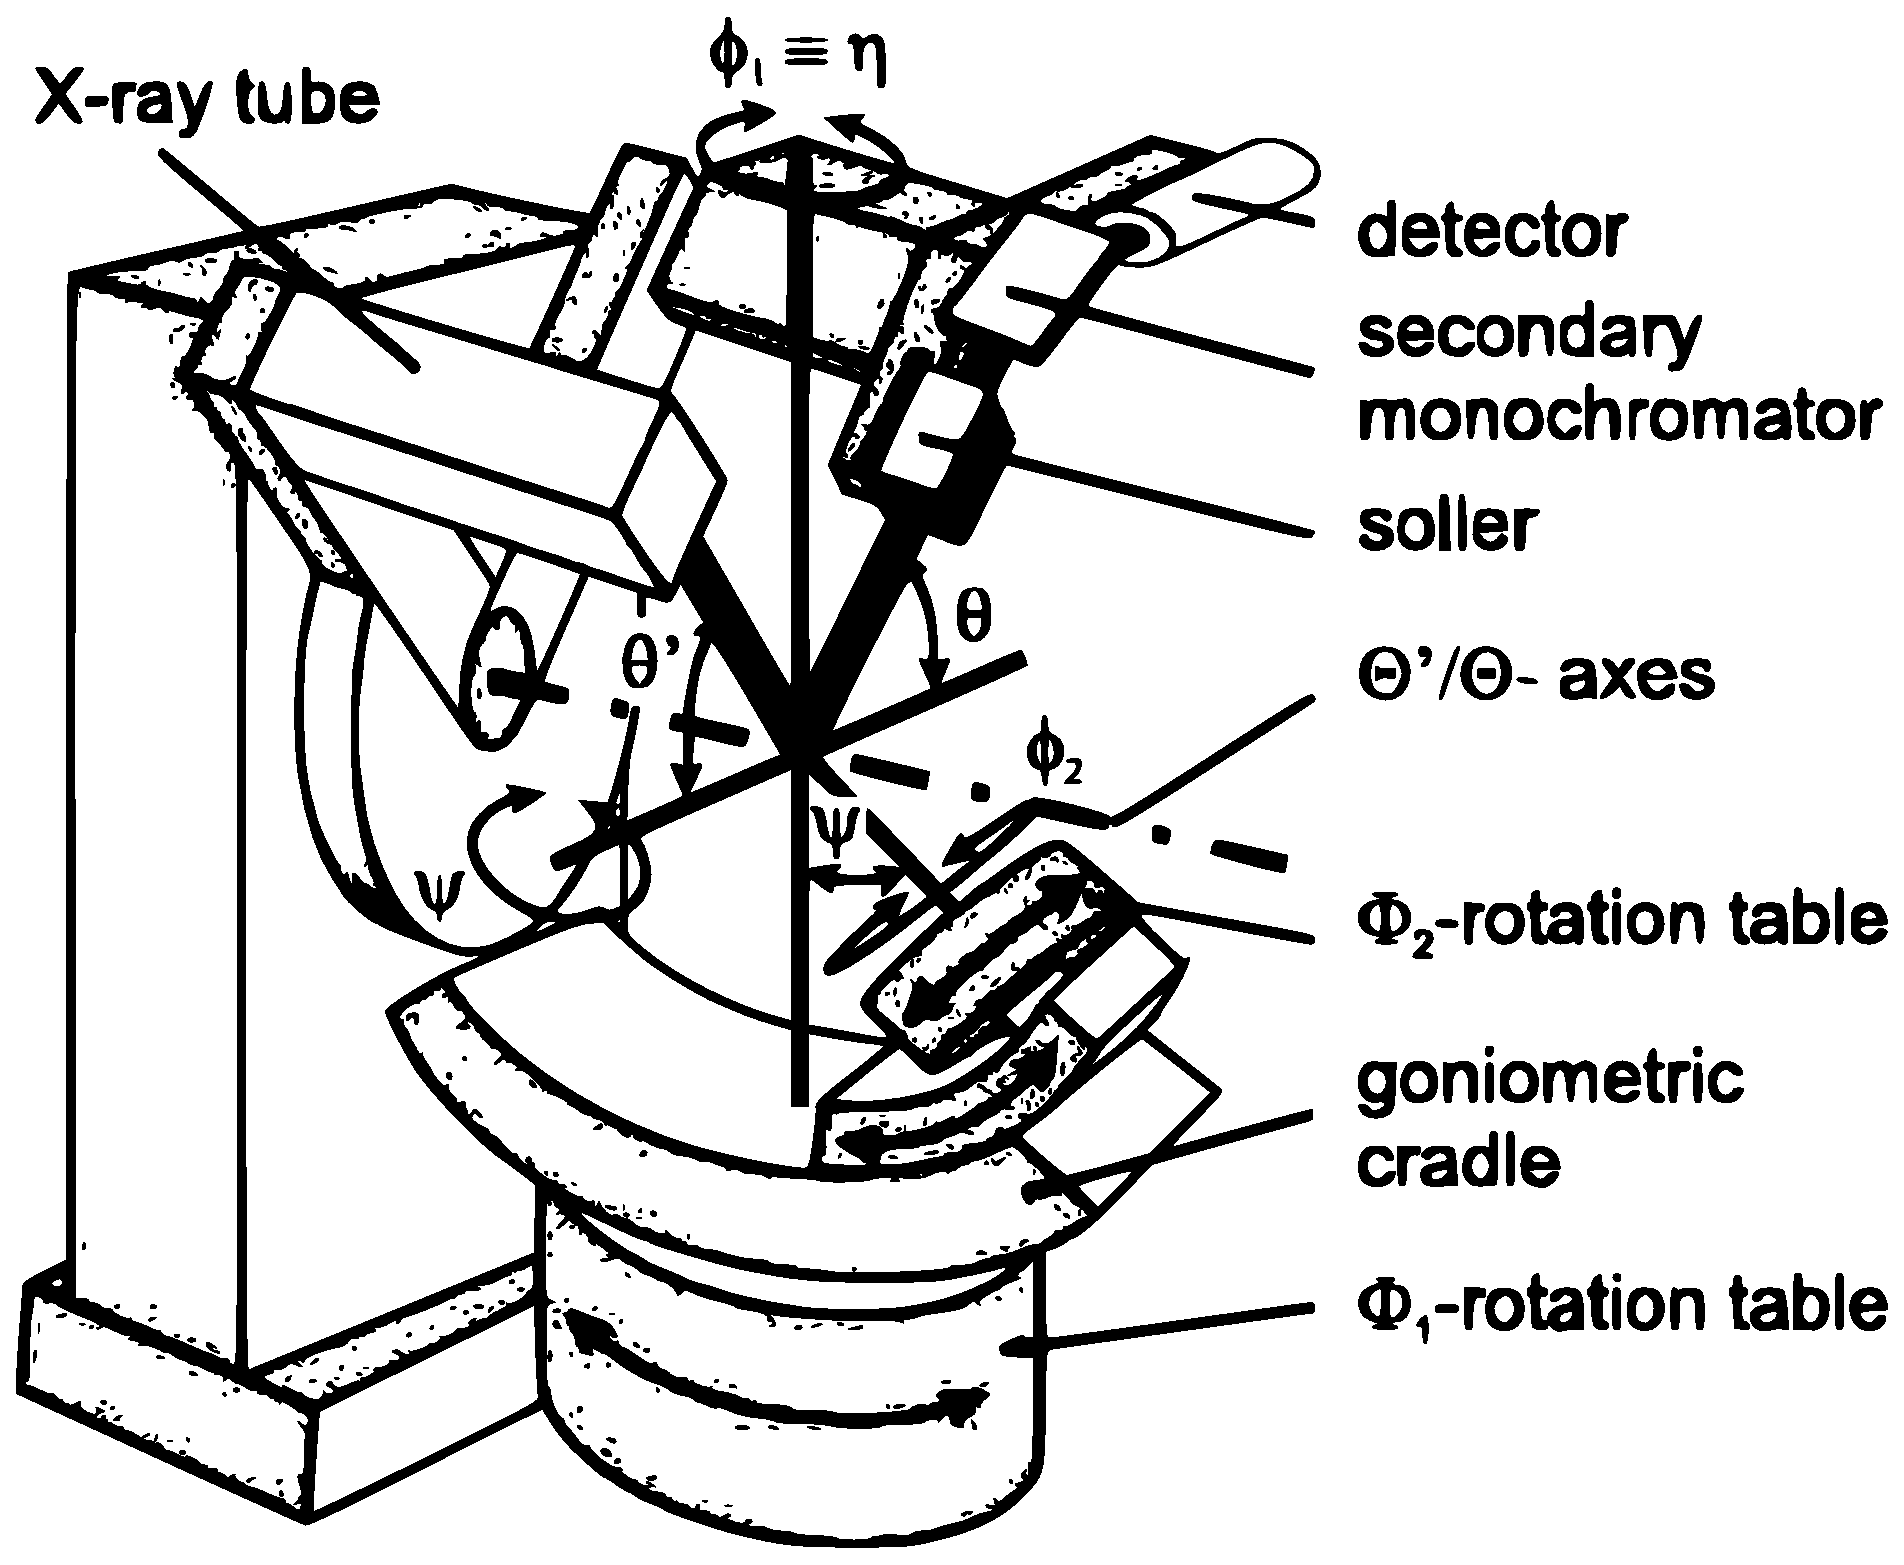
\includegraphics[width=8.5cm]{fig4}
    \caption{\label{tab1}A labeled image of a standard X-ray diffractometer. Adapted from \cite{ref04}.} 
    \end{figure} 
Experimental procedures for X-ray Diffraction involve stabilizing the sample onto the cradle, varying the angle of the X-ray source, and measuring the resulting intensity
values. For each step where the angle of the X-ray source is varied, the sample itself (with the help of the cradle) is oriented in all different directions while the diffraction intensity is measured. This is repeated for all incidient beam angle values.
It's important to recognize that, for any given sample with an unknown single grain orientation, the user must measure across all possible X-ray beam angles (from 0 to 90 degrees) and record the ensuing intensity 
measurement to account for any possible orientation that the grain could be in.

Thus far, the discussion of XRD mechanisms has been focused on measuring a single grain/crystal within a steel sample; however, in order to experience
constructive interference phenomena for the single grain, the single grain itself has to be oriented perfectly with respect to the incoming X-ray source and the
detector. This is a very strict and exact requirement; however, as mentioned earlier,
steels are arranged of thousands of different randomly-oriented grains (polycrystalline). Therefore, regardless of angle of X-ray beam impact, diffraction
phenomena of some sorts can be observed as certain randomly-oriented crystal planes can happen to be positioned appropriately to allow for "clean" diffraction and constructive
interference \cite{ref05}.

\subsection{Interpreting XRD scan results}
The X-ray diffractometer sampling procedure generates XRD scan outputs, which are used to ultimately calculate how much retained austenite 
exists in the steel sample. A sample graph output can be seen in \textbf{Figure 5}, which plots relative measured intensity as a function of
$2\theta$, or twice the incident beam angle.

\begin{figure}[h]
    \centering
    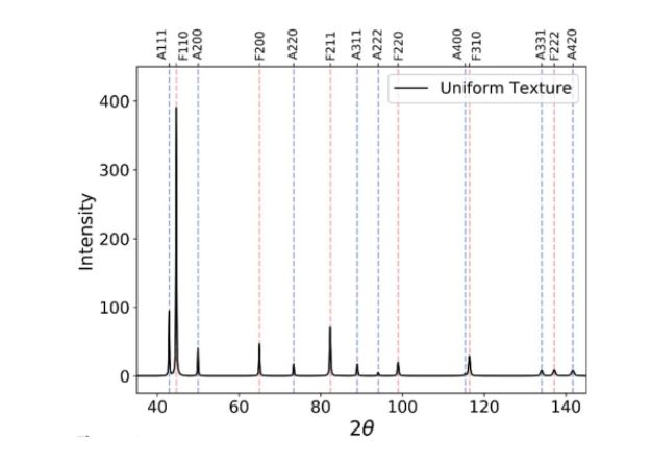
\includegraphics[width=8.5cm]{fig5}
    \caption{\label{tab1}A sample, generic XRD scan output. The 'peaks' of the graph indicate the existence of a
    certain phase at a certain orientation. Adapted from \cite{ref06} with permission.} 
    \end{figure}

The selective appearance of peaks at certain $2\theta$ values implies that those crystal planes oriented at the given $2\theta$ values were conducive to satisfying the 
constructive interference requirement, thus registering as high counts of intensity on the detector. Each phase in the steel sample
produces a unique set of diffraction peaks; the peaks themselves correspond to particular crystal planes. As an important aside, in this project,
Miller indices (sets of 3 numbers which correspond to the orientation of a certain plane defined in 3 different axes - such as the (100) plane) are used as notations for defining
such crystal planes.

As alluded to earlier, different phases of steel differ in the arrangement of atoms in the unit cell structure
(BCC in ferrite vs FCC in retained austenite). Therefore, interplanar distance is a variable that can be very useful to distinguishing 
between different phases in steel, since the different unit cell structures between ferrite and retained austenite imply different values 
for atomic distance (distance between consecutive atoms in a structure). \textbf{Bragg's condition} seen below allows for a relationship between 
incident X-ray beam angle and measured interplanar distance (something that was hinted at in \textbf{Figure 3}), 
assuming the X-ray source produces beams of consistent wavelength:
\begin{equation}
    n\lambda = 2d\sin\theta 
\end{equation}
Where $n$ is any-order integer value, $\lambda$ refers to the wavelength of the X-ray particles, 
$d$ refers to the distance between adjacent crystal planes in the lattice structure, and $\theta$ refers to the
angle of impact of the X-ray beam.
  

   
Assuming crystal planes are all oriented randomly, the calculation of retained austenite from the XRD scan graph is directly correlated to 
the measured intensity values: higher intensities imply that more crystal planes are responsible for creating constructive interference, implying
that a greater volume of a phase is present in the material. Following this reasoning, the relevant "peaks" that correspond to each phase 
are integrated, comapred to values from literature, and ran through a series of functions to calculate theoretical phase fraction value. 

The choice of which peaks to integrate is another variable of interest in this project: the standard choice for retained austenite phase
fraction calculation is a set of 3 peaks; however, this is an arbritrary measure and one that can differ between lab groups. Theoretically,
incorprating all peaks corresponding to a certain phase should allow for the most accurate calculation of phase fraction; however, studying
this variable can allow the discovery of combinations of peaks that can perform considerably better and lead to improved measurement accuracy.
But perhaps most importantly, a critical motivation for researching the effects of this variable will be introduced in the next section, one that especially
operates in the context of the issues that impact phase fraction measurement accuracy.



\section{Crystallographic Texture: Motivations of this research}
\subsection{Introduction into Crystallographic Texture}
The typical calculation of retained austenite phase fraction hinges on the \emph{significant} assumption of the random orientation of crystal planes
within the steel sample; however, this assumption serves to the basis of a host of problems. A round-robin study conducted by \textit{Jacques et. al} 
for conducting retained austenite phase fraction measurements of a fixed sample has shown a complete inability to generate consistent phase fraction values \cite{ref07}. 
The results of the study, as visualized in \textbf{Figure 6}, depict measurements ranging from as low as 3\% to as high as 30\%.

\begin{figure}[h]
    \centering
    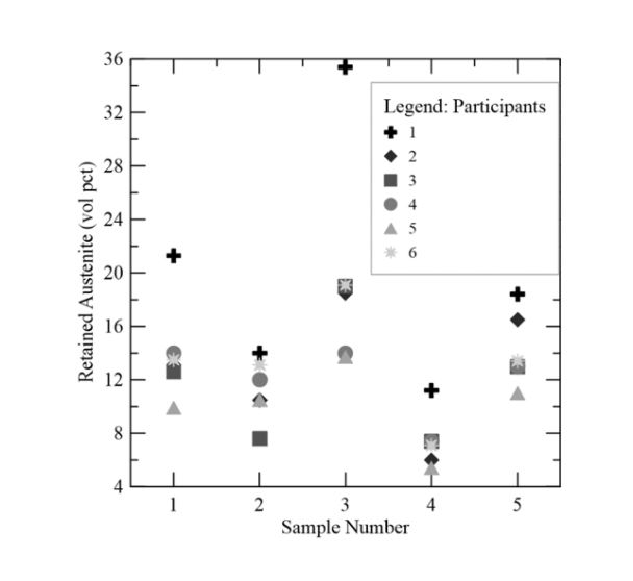
\includegraphics[width=8.5cm]{fig6}
    \caption{\label{tab1}A graph representing the incredible discrepancies in phase fraction measurements of retained austenite 
    in steel samples, by 6 different members. Adapted from \cite{ref07}.} 
    \end{figure}

The suspected culprit for these inconsistent measurements is crystallographic texture, which is a preferred orientation of grains
within a crystal lattice. When grains are in completely random orientation, we say that there's no texture
present, and vice versa. \textbf{Figure 7} provides an intuitive visual comparison of the orientation of crystal planes with texture present
(upper diagram) and texture not present (lower diagram).

\begin{figure}[h]
    \centering
    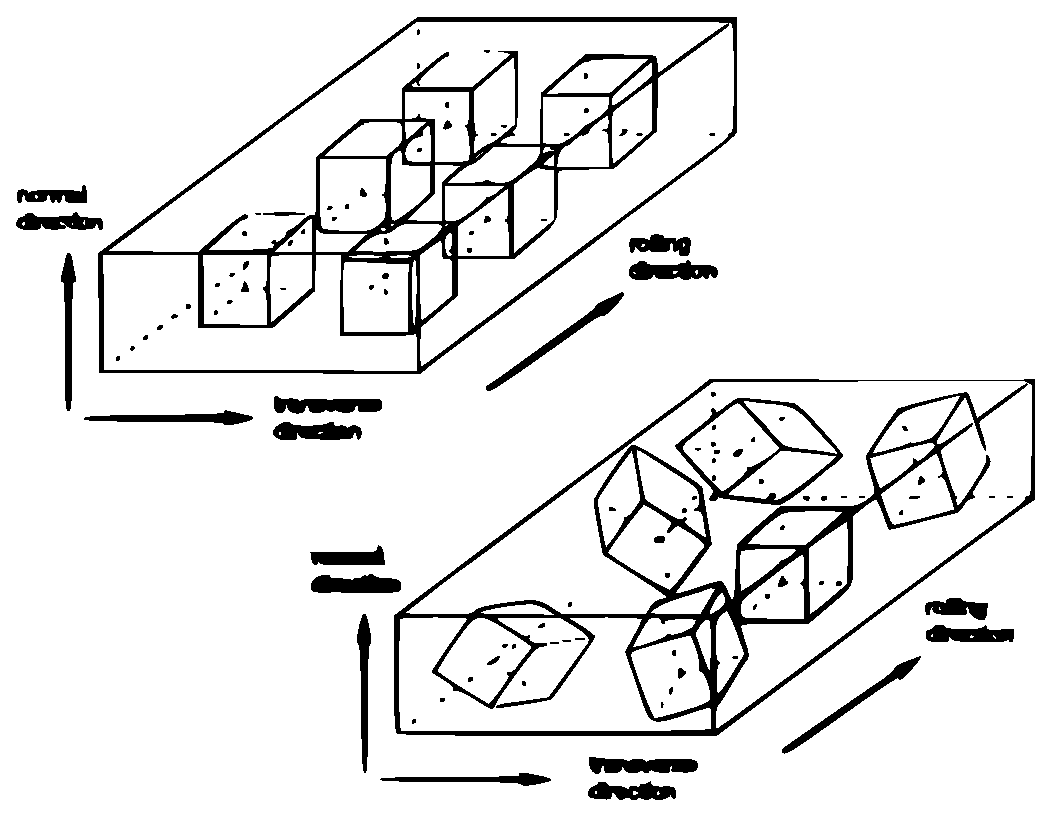
\includegraphics[width=8.5cm]{fig7}
    \caption{\label{tab1}A comparison of crystal orientations in textured materials (top left) and nontextured (random
    mly-oriented crystals) materials (bottom right). Adapted from \cite{ref02}.} 
    \end{figure}

The presence of texture in a steel sample indifcates that certain crystal planes are oriented preferentially in a certain direction 
more or less so than usual (depending on the type of texture). For practical purposes, this can lead to shifts in the measured intensities and $2\theta$
values for the peaks corresponding to lattice planes in the XRD scan graph. Thus, texture can lead to erroneous phase fraction calculation, 
as these calculation steps are dependent on the integrals and locations of specified peaks.

\subsection{Texture Components}
From mechanical rolling of steels to the recrystallization processes in the heating/quenching stage, textures can develop in a 
variety of ways during the thermomechanical processing stage of the steel. For commonly-occurring texture mechanisms, 
there are proper names that have been assigned to them. A \textbf{texture component} is a specific crystal orientation 
that’s heavily prevalent in processed materials. Texture components get their names either from the materials they are 
most prominently found in (Brass, Copper) or the scientists that discover them (Goss) \cite{ref08}. This project focuses on analyzing 20
of the common texture components that can appear in the ferrite or austenite phase; note that this collection isn't exhaustive. 
As an example, \textbf{Figure 8} provides a (heavily simplified) aid for visualizing the "Goss" texture component within a steel sample.
\begin{figure}[h]
    \centering
    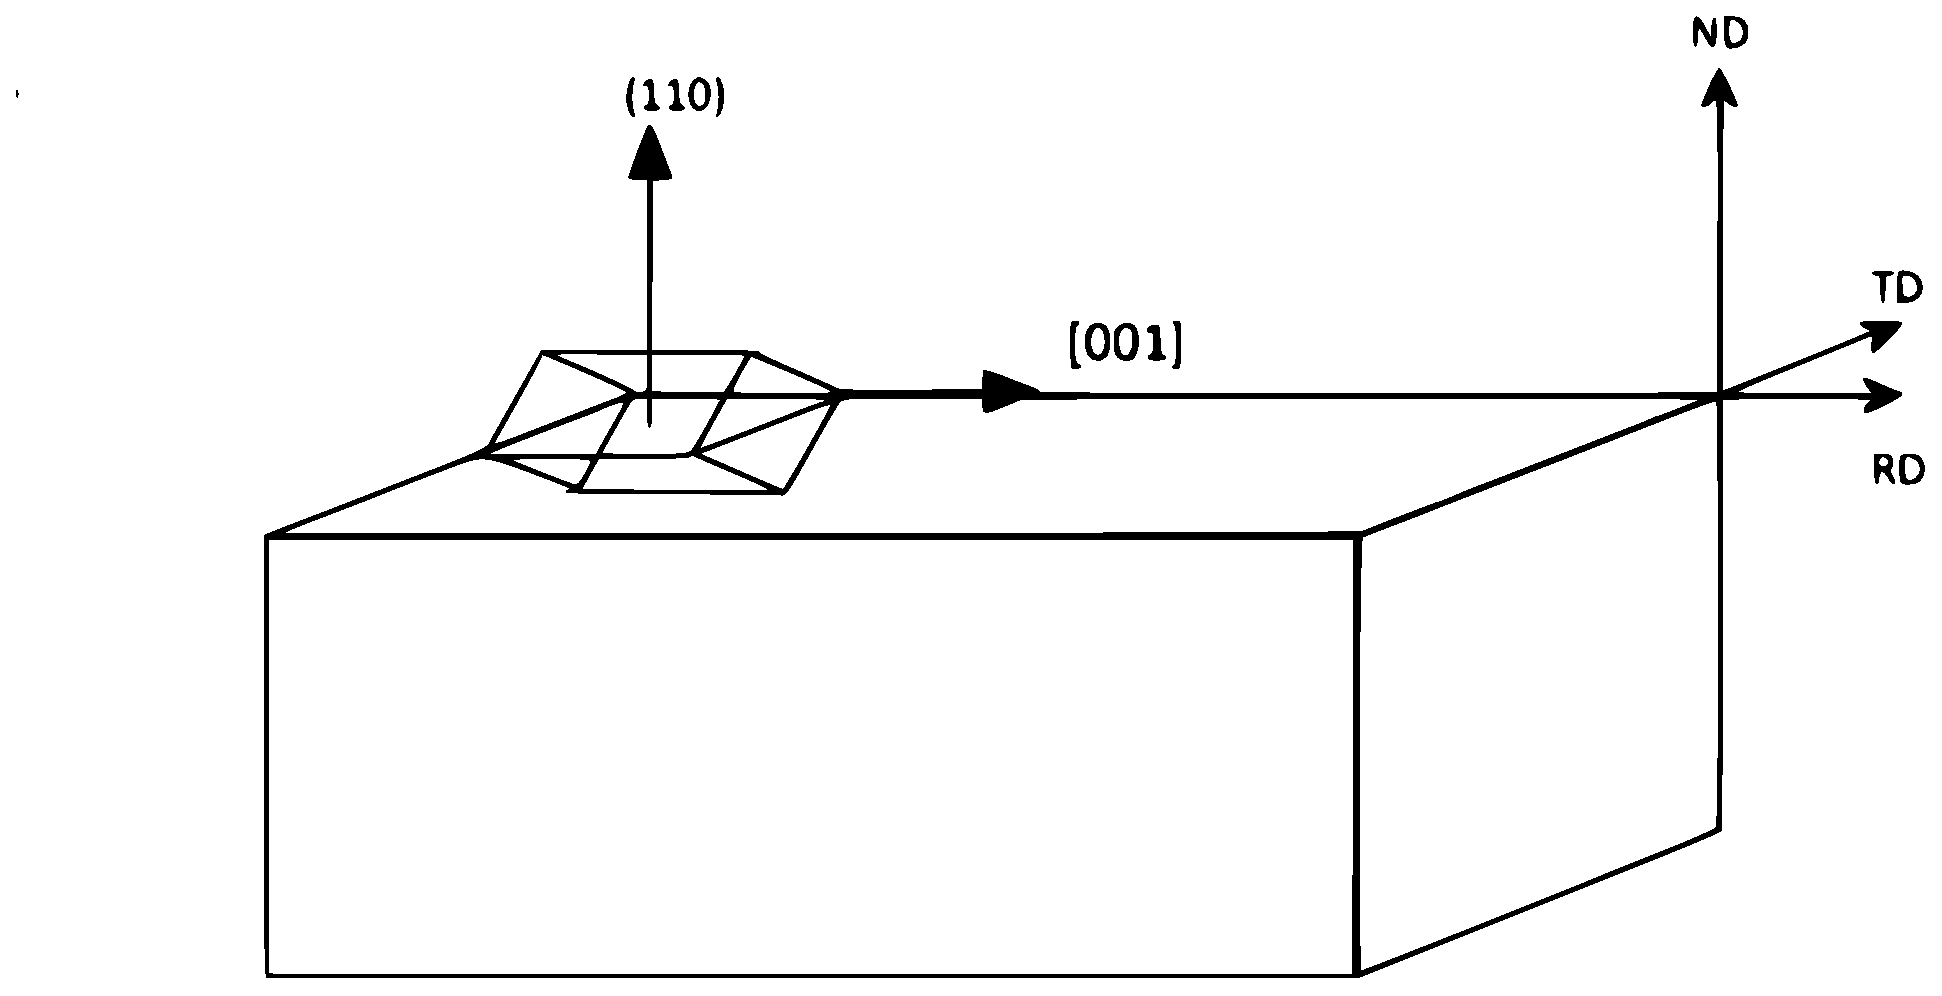
\includegraphics[width=8.5cm]{fig8}
    \caption{\label{tab1}A simplified visualization of the Goss texture component. Adapted from \cite{ref08}.} 
    \end{figure}

Practically speaking, texture present in steels is usually a combination of multiple texture components. Breaking down texture analysis
into individual components allows for ties to be made between the type of steel processing and the formation of a certain texture 
component. In other words, based on knowledge of certain processing conditions, scientists can predict the texture components
present in the material. Understanding which components are present in the steel can allow scientists to appropriately
"weight" the presence of the relevant texture components when trying to analyze the structure and composition of the material.
 

\subsection{The motivations and goals of this research}
As seen above, crystallographic texture can play a significant role causing measurement bias of retained austenite phase fraction \cite{ref06}.
To mitigate these effects, this project focuses on developing new sampling procedures, and testing them for their ability to accurately
capture a known retained austenite phase fraction value (as stated earlier, this project will use 0.25) in the presence of particular texture components.
Furthermore, this project will focus on understanding the relationship between combinations of peaks used from XRD scan graphs and accuracy of the ensuing
phase fraction values. Considering that individual peaks represent crystal planes in a sample, connections can be made between those crystal planes
and the respective orientation of certain texture components. In other words, if a texture component is known to be present in a sample, then an apt choice
of peak combinations can allow for an accurate calculation of theoretical phase fraction value by avoiding the use of that peak/orientation. Thus, the study of peak combinations and texture 
components on new sampling procedures and their effect on phase fraction calculation allows for comprehensive and revealing analysis that can provide
novel insights into effective procedural techniques for phase fraction measurement in textured steels.

\section{Project Methodologies: Visualization Techniques and Sampling Schemes}

The driving force needed to answer such research questions lies in the concept of sampling schemes; however, before the specifics of each scheme can be discussed, 
quick context into the setup of this research, necessary background topics, and previous research in this field will be provided.

\subsection{The setup of this project}
For reasons tied to both COVID-19 protocols and for practical purposes, this project is being approached computationally and remotely.
A simulation of the XRD process has been provided, and the code needed to convert intensity values outputted from the mentioned XRD simulation scan into phase fraction values has already been developed. 
The focus of the project involves the development of new sampling schemes (through Python), and an evaluation of the results returned by the simulation. ultimately, the computational stage 
(in a broader sense) will allow us to flag schemes that performed well in the simulation; in the future, the plan is to run physical XRD scans using the flagged promising sampling methods to see how well 
they can remove such measurement bias.

In this stage of computational prototyping, there is sizable benefit to being able to visualize individual aspects of this project, from texture components and
specific sample orientations to the sampling schemes themselves. To accomplish this, pole figures are implemented to provide an intuitive and rather 
straightforward representation of these topics. The section below will quickly provide an introduction into the implementation and purposes of pole 
figures in this project.

\subsection{Introduction into Pole Figures and Density Contour Plots}
Briefly speaking, \textbf{pole figures} are a means to visualize crystallographic texture. They offer an intuitive visual representation
of the orientation of various crystal planes in the sample. In this project, pole figures are used to visualize
sampling procedures and texture components. Both these figures have different mechanisms connected with their 
different respective purposes.

To begin, it's important to recognize that the XRD scan process is inherently 3-dimensional. Imagine taking the steel sample to be scanned
and enveloping it evenly by a reference sphere. For metallurgical applications, the 3 axes of notation for this sphere are the ND 
(the ‘Normal’ Direction – the one pointing straight up towards the ceiling), RD (the ‘Rolling’ 
Direction – running parallel to the surface where the sample is kept), and TD (the ‘Transverse 
Direction’ – the axis that runs perpendicular to the RD axis on the plane of the table). \textbf{Figure 9} provides a helpful visualization 
of these descriptions.
\begin{figure}[h]
    \centering
    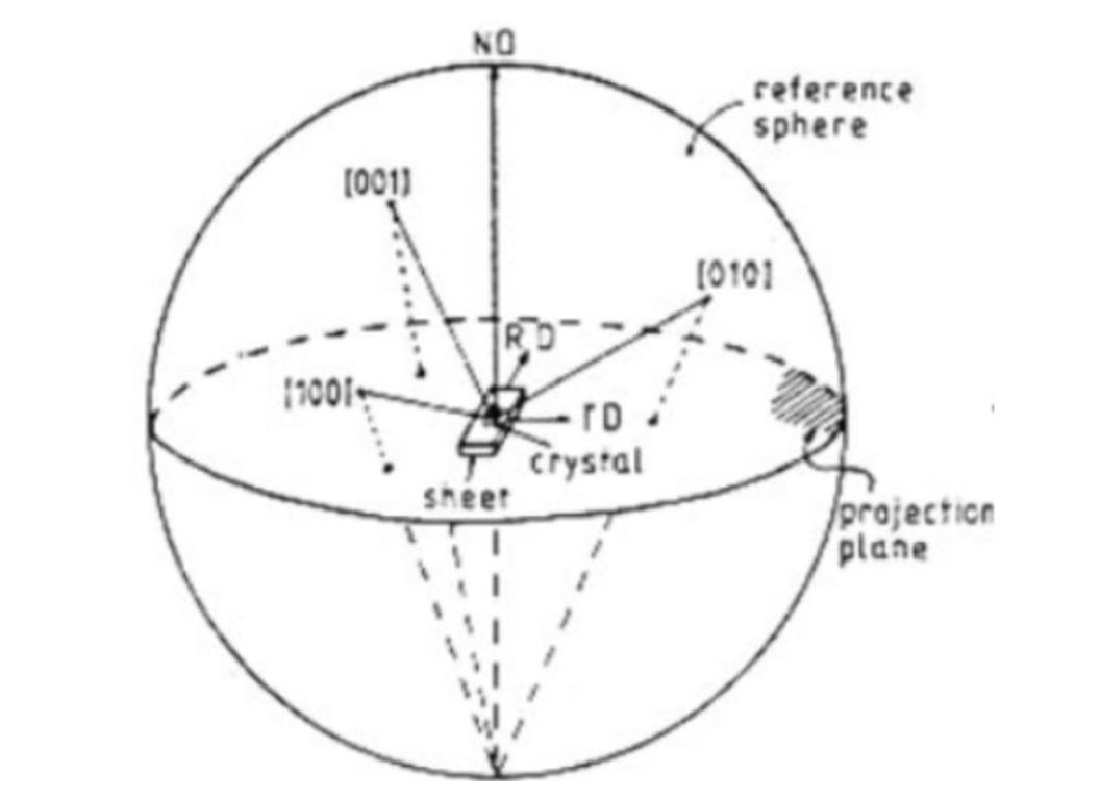
\includegraphics[width=8.5cm]{fig9}
    \caption{\label{tab1}A plot clarifying the 3 axes of notation in this project. Adapted from \cite{ref09}. } 
    \end{figure}

Next, for a specific crystal plane, imagine drawing a vector originating from the center of our reference sphere, called a \textbf{plane normal}. This plane normal is orthogonal
(perpendicular) to the surface of the crystal plane, and eventually intercepts the surface of the sphere (which can be fundamentally understood in \textbf{Figure 9}). The point of interception can be
represented as a coordinate point, whose location is parametrized by the spherical angles declination ($\chi$) and azimuth ($\phi$). 
Declination, or $\chi$, stands for the “tilt,” or the angle the plane normal makes with respect to the ND. 
Azimuth, or $\phi$ on the other hand, stands for the “rotation,” or the angle the  
plane normal makes on the RD-TD plane (counterclockwise convention). To clarify such conventions, \textbf{Figure 10} provides a labeling 
of both these spherical angles.
\begin{figure}[h]
    \centering
    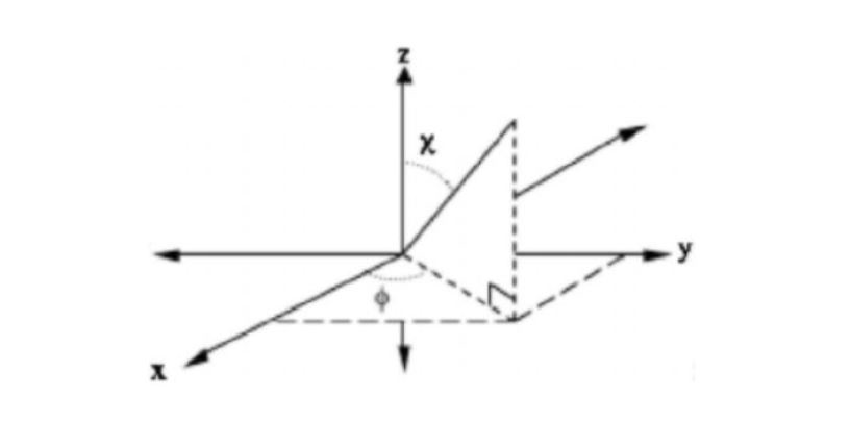
\includegraphics[width=8.5cm]{fig10}
    \caption{\label{tab1}A plot defining the notations of tilt ($\chi$) and rotation ($\phi$). Adapted from \cite{ref10}.} 
    \end{figure}

Across multiple orientations, a pole figure plot can be generated. Following the plotting pattern shown back in \textbf{Figure 9}, a pole figure plot 
for those 3 beams can be generated, as seen in \textbf{Figure 11}.
\begin{figure}[h]
    \centering
    
\includegraphics[width=8.5cm]{fig11}
    \caption{\label{tab1} The pole figure result from the scanning followed in \textbf{Figure 9}. As a side note, 
    the orientations for RD and TD are switched from the conventional axes labeling, but the idea remains the same. Adapted from \cite{ref09}.} 
    \end{figure}

Pole figures can be used for both visualizing textures and sampling schemes. Although both of these applications deal with 
fundamentally different values/concepts, a consistent utility in mapping plot density exists among both applications. Because analysis of texture from pole figures involves studying the relative density of sampling points/normalized intensities values, 
this project uses \textbf{density contour plots} to quantitatively represent regions of uneven sampling in the pole figure. A sample density
contour plot (for a scheme called the "Equal Angle Scheme" -- to be elaborated upon later) can be seen in \textbf{Figure 12}:

\begin{figure}[h]
    \centering
    \includegraphics[width=8.5cm]{fig12}
    \caption{\label{tab1}A density contour plot of the Equal angle scheme. 
    This representation provides an added quantitative dimension for analyzing oversampling and undersampling in the pole figure.} 
    \end{figure}



\subsubsection{Visualizing Texture Components}
Filler section 


Tables are done as follows:
\begin{table}[h]
    \begin{tabular}{||c c c||}
    \hline
    \textbf{Peak Pair} & \textbf{R. Austenite Planes} & \textbf{Ferrite Planes} \\ [0.5ex] 
    \hline\hline
    \emph{1 Pair-A} & (111) & (110) \\ 
    \hline
    \multirow{2}{*}{\emph{2 Pairs-A}} & (200) & (200) \\
    & (220) & (211) \\
    \hline
    \multirow{2}{*}{\emph{2 Pairs-B}} & (200) & (200) \\
    & (311) & (211) \\
    \hline
    \multirow{3}{*}{\emph{3 Pairs-A}} & (200) & (200) \\
    & (220) & (211) \\
    & (222) & (310) \\
    \hline
    \multirow{3}{*}{\emph{3 Pairs-B}} & (200) & (200) \\
    & (220) & (211) \\
    & (311) & (220) \\
    \hline
    \multirow{3}{*}{\emph{3 Pairs-C}} & (111) & (110) \\
    & (200) & (200) \\
    & (220) & (211) \\
    \hline
    \multirow{4}{*}{\emph{4 Pairs}} & (111) & (110) \\
    & (200) & (200) \\
    & (220) & (211) \\
    & (311) & (220) \\
    \hline
    \multirow{5}{*}{\emph{5 Austenite, 4 Ferrite}} & (111) & (110) \\
    & (200) & (200) \\
    & (220) & (211) \\
    & (311) & (220) \\
    & (222) & N/A (only 4 used) \\

    \hline
    \multirow{8}{*}{\emph{MaxUnique}} & (111) & (110) \\
    & (200) & (200) \\
    & (220) & (211) \\
    & (311) & (310) \\
    & (331) & (222) \\
    & (420) & (321) \\
    & (422) & N/A \\
    & (511) & N/A \\
    \hline
   \end{tabular}
   \caption{A table summarizing the reflection planes used in specific peak combinations. The planes are organized by
   the phase they are associated with (Retained Austenite or Ferrite). Entries labeled 'N/A' for certain columns act as a placeholder to preserve the symmetry of the table. 
   }
\end{table} 


\subsubsection{Visualizing Sampling Procedures}
For visualizing sampling procedures, each of the spherical coordinates of the plane normal that intercepts the reference 
sphere is recorded for all possible sample orientations.
With all the different (tilt, rotation) coordinates, we can now plot 
each of these coordinate points on a pole figure which would be oriented with respect to the normal direction \cite{ref09}.
Conceptually, each of these points represent the diffraction vectors in the XRD scanning process, each of which are 
associated with a particular sampling orientation. 

The focus of this project in particular largely boils down to the sampling procedures themselves. The reasoning behind tackling 
texture-induced measurement bias by changing sample orientation is simple: if the sample itself is "randomly" oriented (tilted at various angles, rotated
at various angles), this can represent measurement of a random set of orientations, thereby ensuring that regions of preferential 
alignment of crystals are not oversampled, and vice versa.

There are different methods used to
measure diffraction intensities across various different sample orientations. For example, the rate at which the tilt of the sample
specimen is changed, the increments of sample rotation, etc. can all be varied to study how well a particular set of sampling conventions
mitigate measurement bias caused by texture. These sets of sampling conventions (specific set of tilt and rotation coordinates that
prescribe the orientation of the sample) are called \textbf{sampling schemes}. Such sampling schemes can be visualized easily through pole figures, and 
as alluded to earlier, predictive statements outlining the performance
of each sampling scheme can be made based on how evenly and uniformly the sampling coordinates are distributed over the pole figure grid. The section below will
outline each of the schemes that were implemented and tested in this project.
 

\subsection{Discussion of Sampling Schemes in this Project}
This project focuses on developing 4 of such novel sampling schemes and testing them for their ability to mitigate phase fraction 
measurement bias. The evaluation of the performance of a sampling scheme in this project hinges on two factors: measurement accuracy (how well each scheme can measure the 
0.25 retained austenite phase fraction value in the presence of multiple texture components), and number of sampling points used. Although complete and even coverage of the pole 
figure is the primary objective of any developed scheme, reduced sampling points for these schemes is also a preferable goal for obvious reasons (reduced sampling time).


Of course, the development, implementation, and testing of sampling schemes is not a novel field. The section below will cover a brief 
history of sampling schemes, starting with conventional sampling methods and the most promising sampling schemes to date.


\subsubsection{The Equal Angle Scheme}
Traditionally, XRD procedures for varying sample orientation involved rotating the sample in even increments (upto 360 degrees), 
then tilting the sample by the very same increment, and repeating the rotation process again until the maximum tilt was reached
(90 degrees). This procedure is called the \textbf{Equal Angle Scheme}, getting its name from the even degree increments in tilt and rotation.
Typically, increments of 5º are used for our purposes, given that this value does a good job tackling smoothly-varying textures.
A sampling pole figure for the equal angle scheme can be seen in \textbf{Figure 13}.

\begin{figure}[h]
\centering
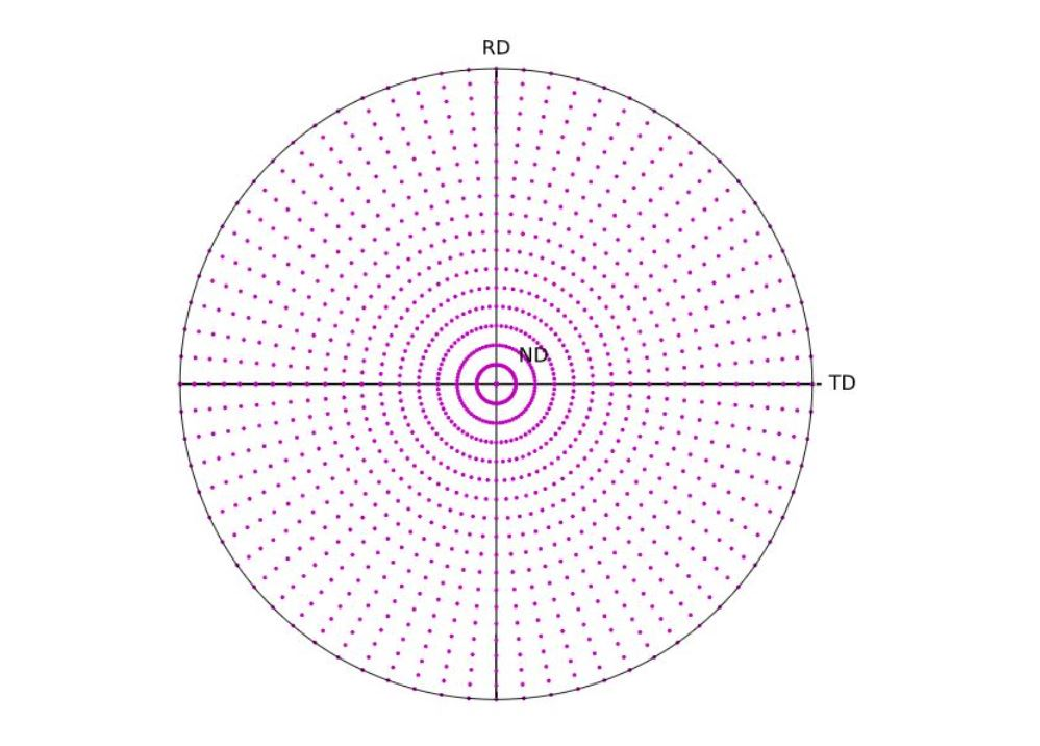
\includegraphics[width=8.5cm]{fig13}
\caption{\label{tab1}A pole figure representation of the Equal Angle Scheme. 
Notice the heavy oversampling along the ND axis and undersampling towards higher tilts.} 
\end{figure}

However, with such simplicity comes significant problems. As visualized back in \textbf{Figure 13}, regardless of tilt value, 
each ring in the scheme will sample 360$^{\circ}$/5$^{\circ}$= 72 points. At low tilt values, there is major oversampling towards the center of the pole figure, 
and undersampling towards the outer edges of the pole figure (where the tilt is highest). This can be visualized by the corresponding
density contour plot for the equal angle scheme (which can be referenced back in \textbf{Figure 12}).

For this reason, the 
Equal Angle scheme doesn’t do a great job mitigating measurement bias caused by texture, because of the evident 
uneven distribution of sampling points throughout the pole figure. 

Another issue with the equal angle scheme pertains to the sheer amount of points being sampled (nearly 1400, to be exact). To tackle both objectives of excellent
measurement accuracy and reduced sampling time, 
a novel variation of the Equal-Angle scheme was proposed, 
called the “CLR scheme.” The section below will discuss the implementation details and theory behind the CLR grid.

\subsubsection{CLR Scheme}
“CLR” stands for “constant local resolution,” the idea being that 
the rotation increment between consecutive sampling points asymptotically approaches the 
value of the tilt increment as the tilt value approaches its maximum \cite{ref11}. As implied in the previous section, the theory of the CLR grid
is to address the significant oversampling along the Normal Direction axis by decreasing the rotation increment for increasing tilt values.
A sample pole figure of the CLR grid can be seen in \textbf{Figure 14}, demonstrating the above concepts.
\begin{figure}[h]
    \centering
    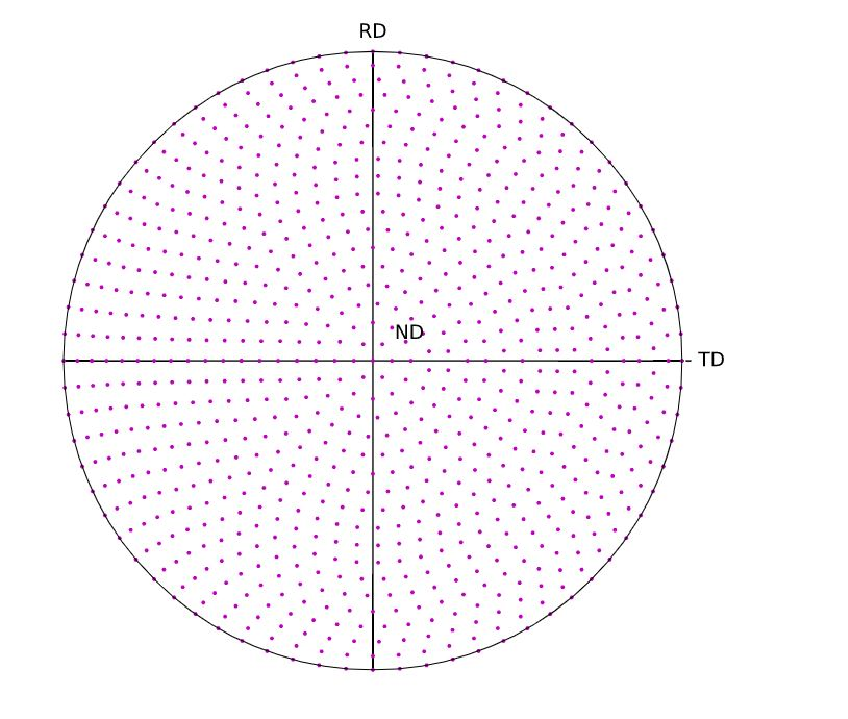
\includegraphics[width=8.5cm]{fig14}
    \caption{\label{tab1}A pole figure representation of the CLR scheme. Notice, as you approach maximum tilt values, 
    the incremental rotation step decreases towards the value of the tilt rotation step.} 
    \end{figure}

A snippet of the algorithm used to implement the CLR grid can be seen in \textbf{Figure 15}.
\begin{figure}[h]
    \centering
    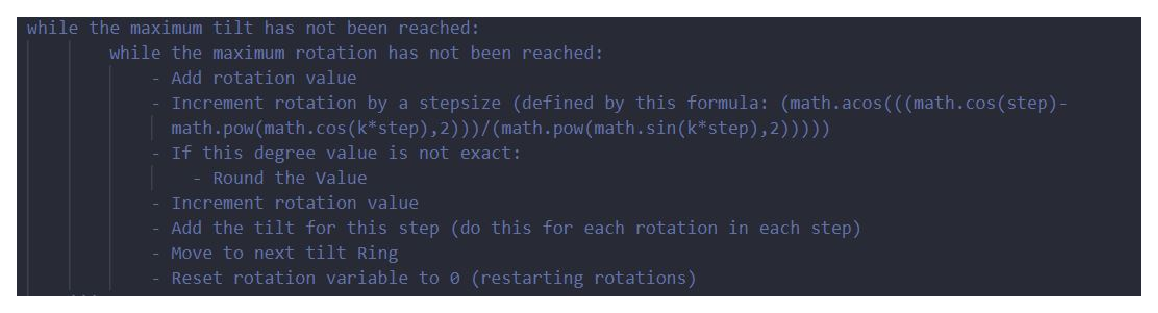
\includegraphics[width=8.5cm]{fig15}
    \caption{\label{tab1}Pseudocode explaining the algorithm used to generate each of the sampling coordinates (in spherical angles) for the 
    CLR grid. Inspired by \cite{ref11}} 
    \end{figure}
 
After successful implementation, it was noted that the CLR grid samples nearly 850 points, which is significantly lower than the 
roughly 1400 sampling points of the equal angle scheme. Furthermore, the CLR grid provides a much more even distribution of sampling points
across the pole figure, with no regions of major oversampling or undersampling, as confirmed by the density contour plot of this scheme in \textbf{Figure 16}.
\begin{figure}[h]
    \centering
    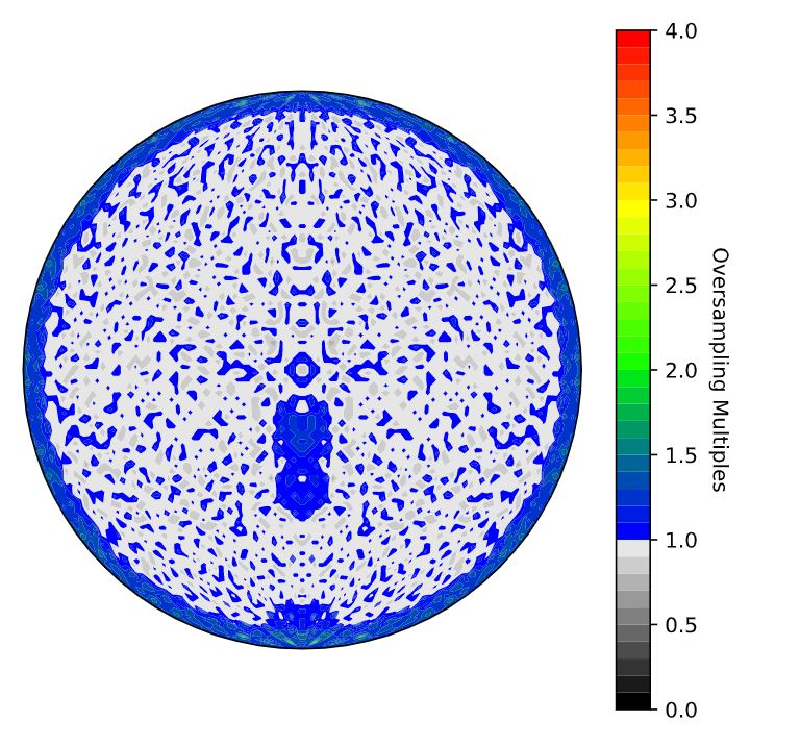
\includegraphics[width=8.5cm]{fig16}
    \caption{\label{tab1}A density contour plot for the CLR grid. Overall, the scheme seems to sample fairly evenly across all orientations.} 
    \end{figure}

Although the CLR scheme does a good job of addressing both of our defined benchmarks (sampling around 850 points, admirable measurement accuracy), 
there is room for improvement. The gold standard for schemes in this research is the hexagonal (hex) scheme, with sampling points arranged in a hexagonal pattern. The section below 
will offer more details of the implementation and details of the hex scheme.

\subsubsection{Traditional Hexagonal Scheme}
From previous research, hexagonal (hex) schemes were one of the most promising sampling procedures to be studied 
and implemented for their ability to achieve promising combinations of phase fraction measurement accuracy
and reduced sampling points. The inspiration for hex schemes came from attempts to cover pole figure grids 
with simple geometric shapes 
as efficiently and completely as possible \cite{ref12}. Through a bit of trial and error, researchers determined that
mimicking a hexagon-shaped distribution of sampling points would provide both a complete coverage of the
pole figure and a consistent, even “resolution” of sampling points throughout the pole figure. A sampling pole figure grid
of a traditional hex scheme can be seen in \textbf{Figure 17}.

\begin{figure}[h]
    \centering
    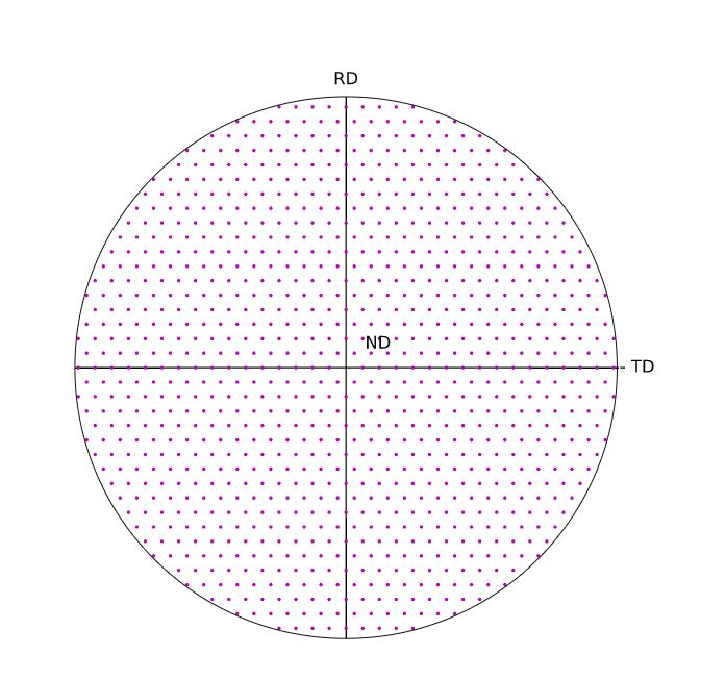
\includegraphics[width=8.5cm]{fig17}
    \caption{\label{tab1}A pole figure for the traditional hex scheme. Overall, it covers the pole figure both evenly and with
    excellent resolution needed to tackle smoothly-varying textures. Inspired by \cite{ref13}.} 
    \end{figure}

In line with the impressive and even sampling of the hex grid, \textbf{Figure 18} provides the density contour plot of the same 
traditional hex scheme.

\begin{figure}[h]
    \centering
    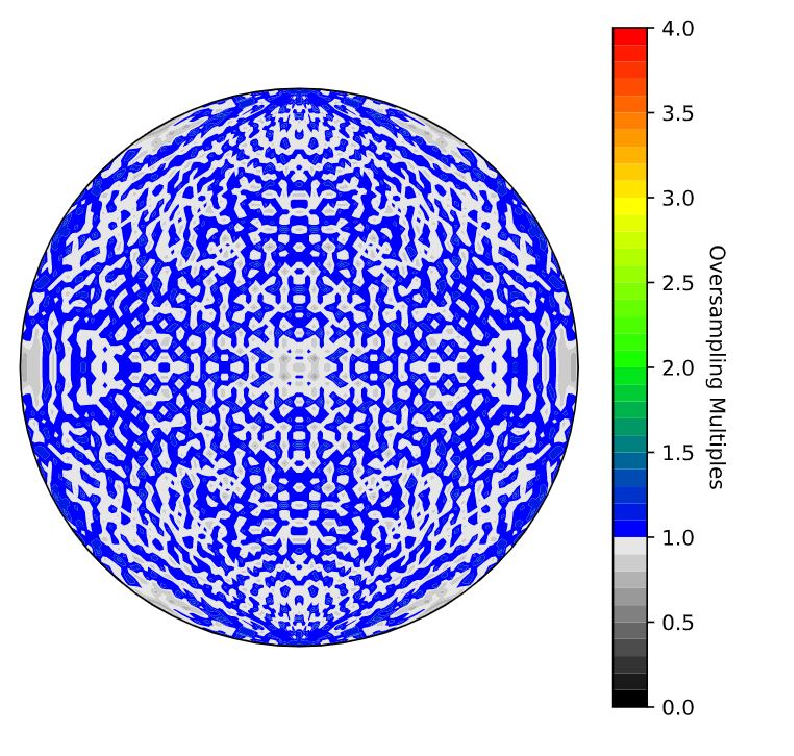
\includegraphics[width=8.5cm]{fig18}
    \caption{\label{tab1}The density contour plot representation of the traditional hex scheme. So far, this is the closest to sampling scheme perfection in terms of even sampling of the pole figure, 
    as evidenced by the heavy coverage of “blue” throughout the figure.} 
    \end{figure}

The fairly complete distribution of blue across the contour plot indicates that the hex scheme samples randomly
and uniformly across all sample orientations, allowing it to achieve incredible phase fraction measurement accuracy.

Still, there’s always room for improvement. While the above traditional hex scheme samples nearly 900 points, 
a newer variation of the hex scheme (called BT8\_Hex) samples nearly half as many points while maintaining a generally-even 
sampling of the pole figure. Next, this report will dicuss the details of the BT8\_Hex scheme \cite{ref12}.


\subsubsection{BT8\_Hex Scheme}
The BT8\_Hex scheme seeks to combine the best of both worlds: reducing the number of sampling points by half while maintaining the 
trademark measurement accuracy of the traditional hex grids. Employing the base trigonometric concepts used in the traditional hex scheme, the BT8\_Hex's implementation
details can be clarified in the pseudocode seen in \textbf{Figure 19}.
\begin{figure}[h]
    \centering
    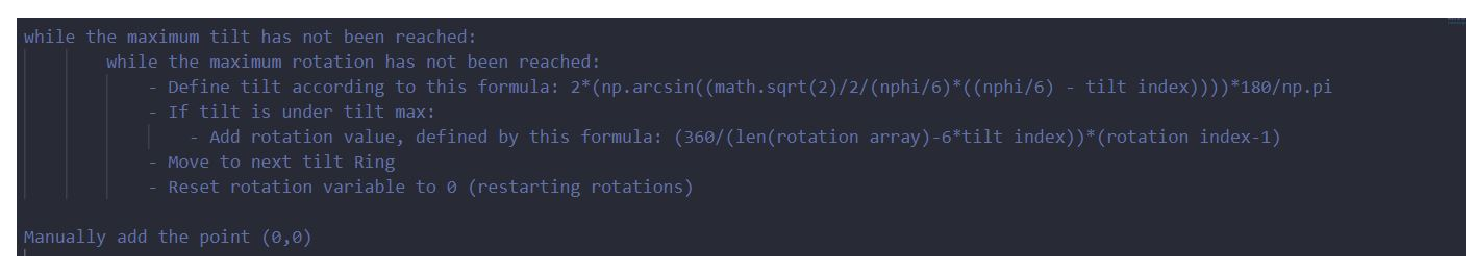
\includegraphics[width=8.5cm]{fig19}
    \caption{\label{tab1}Pseudocode outlining the steps needed to generate spherical angle coordinates for each sampling vector 
    for the BT8\_Hex scheme. Inspired by \cite{ref12}} 
    \end{figure} 

While keeping a similar general structure of a hexagon-patterned sampling
distribution, the BT8\_Hex reduces the resolution/concentration of points, thereby incorporating fewer sampling orientation coordinates
while covering the same pole figure grid area. \textbf{Figure 20} and \textbf{Figure 21} provide the pole figure representation and density
contour plot of this scheme, respectively.

\begin{figure}[h]
    \centering
    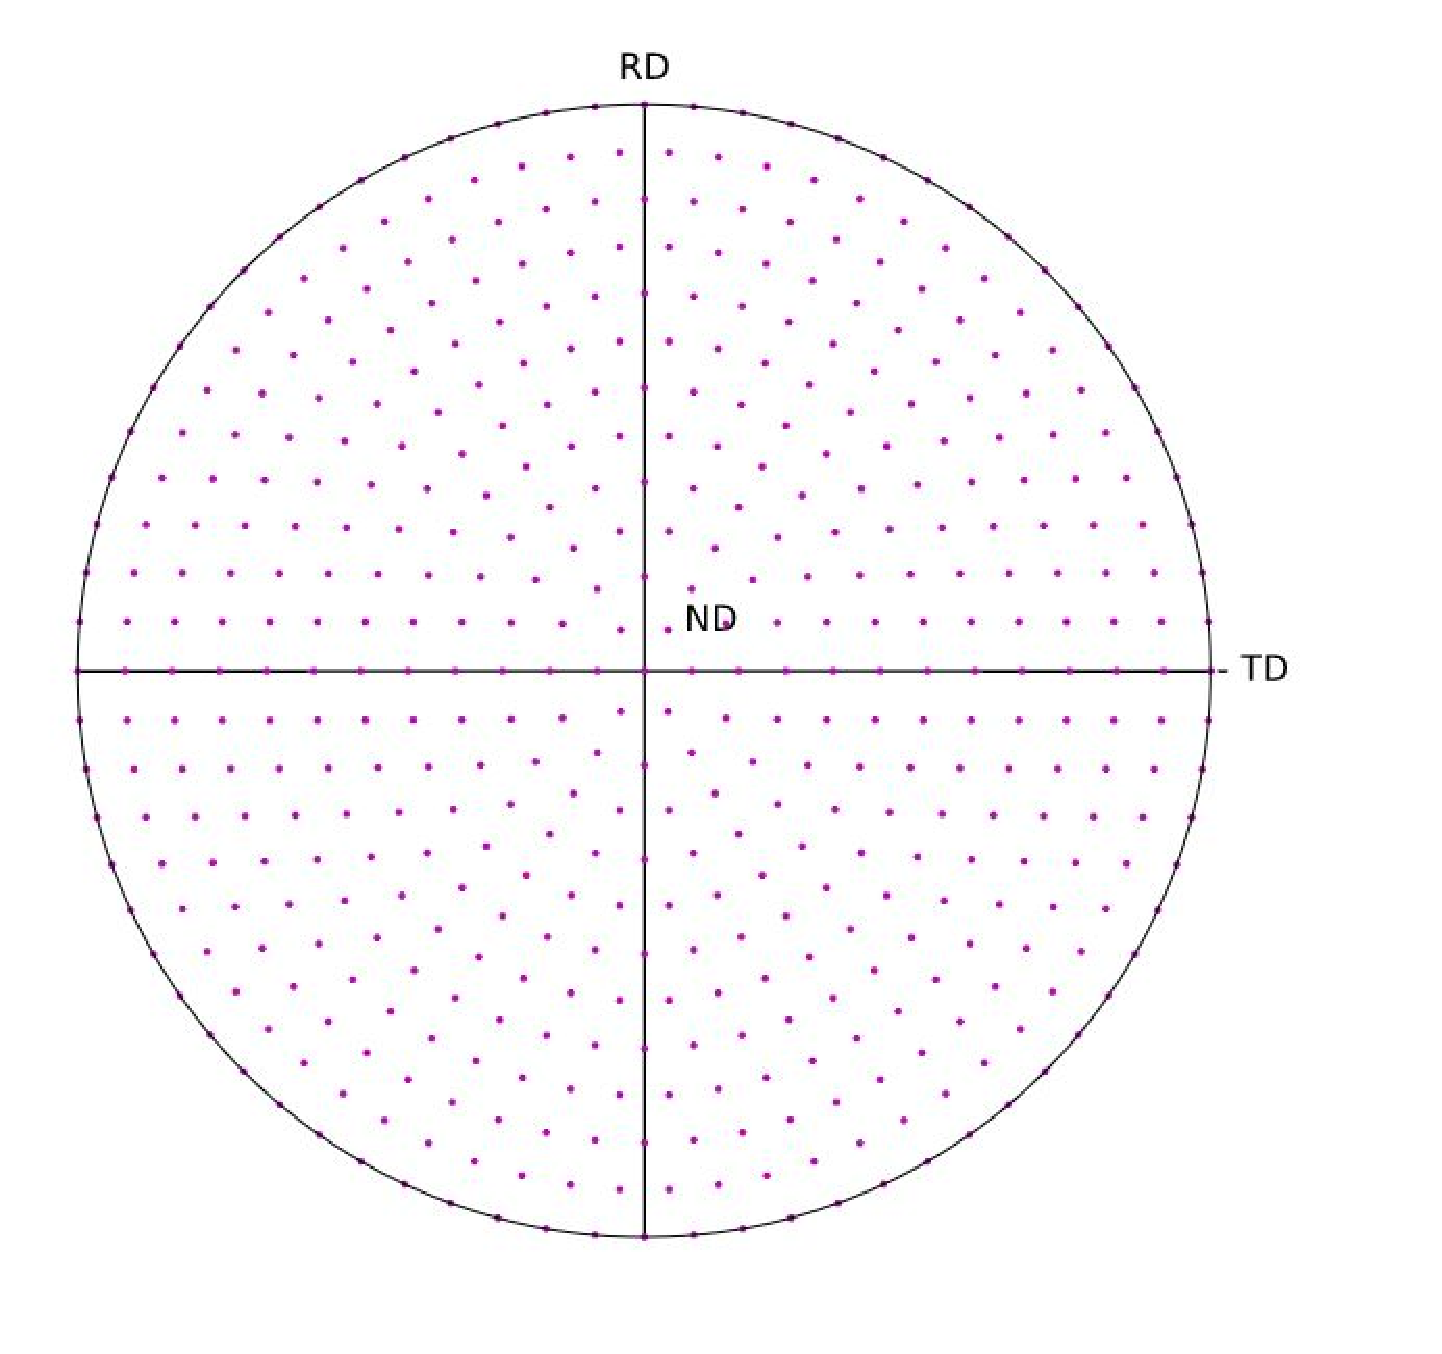
\includegraphics[width=8.5cm]{fig20}
    \caption{\label{tab1}The pole figure representation of the BT8\_Hex grid.} 
    \end{figure}

\begin{figure}[h]
    \centering
    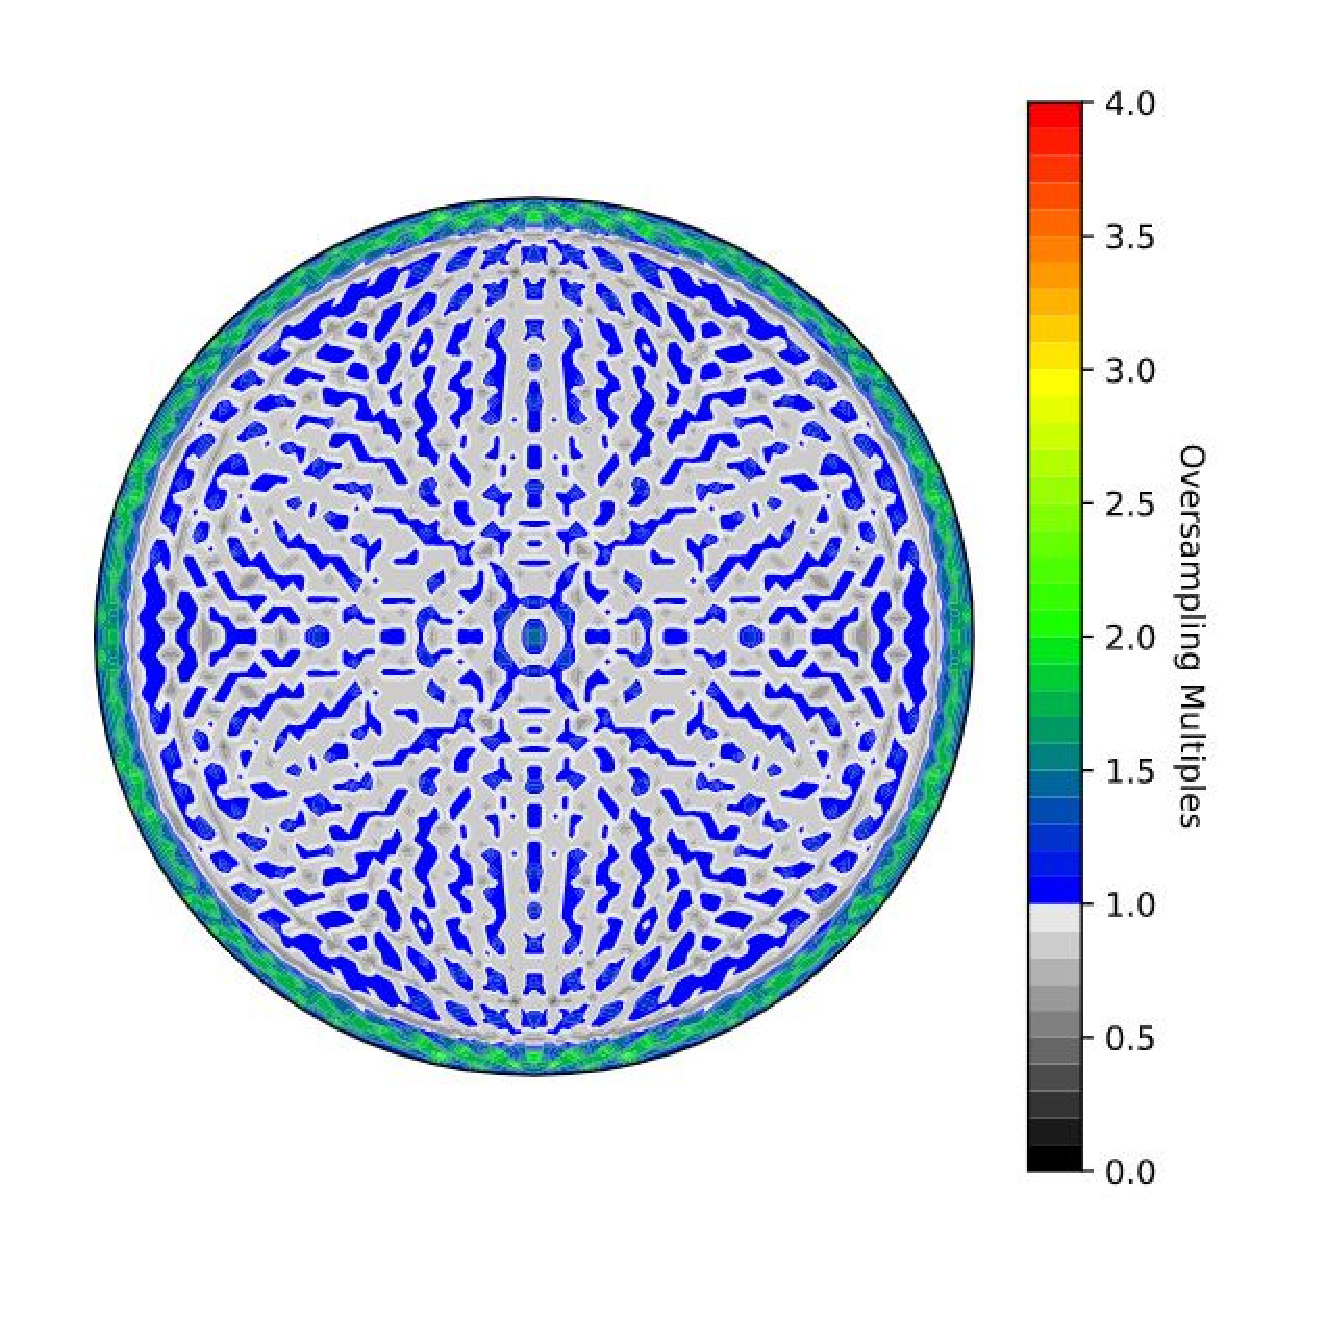
\includegraphics[width=8.5cm]{fig21}
    \caption{\label{tab1}The density contour plot for the BT8\_Hex scheme. Notice the oversampling observed near areas of maximum tilt, 
    but otherwise an even coverage of sampling points throughout the pole figure.} 
    \end{figure}

The most significant detail noticed in these plots is the apparent oversampling at higher tilt values, to a factor of 2. Although the rest
of the scheme is fairly evenly sampled, the abundance of sampling diffraction vectors in regions of higher tilt could provide a significant 
cause of phase fraction measurement bias, in the presence of particular texture components. This is a noteworthy observation to keep in mind,
especially in the evaluation of scheme performance and scan results.

\section{Analysis and Discussion of Results}
After understanding the implementation details and sampling patters of the 4 sampling schemes in this project, an analysis 
and discussion of the results of each scheme can be provided regarding their ability to mititgate phase fraction measurement
bias in the presence of multiple texture components. For this research, heatmaps are used to efficiently view such results. This section
makes use of such heatmpas to evaluate sampling scheme performance against each other and peak combination impact on phase fraction
measurement accuracy. Firstly, however,
the details of the heatmap and how it is used in this project will be provided.
\subsection{Understanding Heatmaps}
The simulation process involves significant amounts of data, making the need for a rapid and effective representation of results apparent. To that end, Heatmaps allow for a straightforward understanding of the impact of the presence of 
various texture components on phase fraction measurement accuracy. A sample heatmap (of the Equal Angle Scheme) can be seen in \textbf{Figure 22}.

\begin{figure}[h]
    \centering
    \includegraphics[width=10cm]{fig22}
    \caption{\label{tab1}A sample heatmap displaying Phase Fraction Calculations for the Equal-Angle Scheme.} 
    \end{figure}

Data is represented in a rectangular fashion; the individual values themselves are depicted by color and shade, offering a quick, intuitive "snapshot" of the simulation results behind 
a given sampling scheme under certain parameters. Each cell/element of the data corresponds to the intersection of 2 individual texture components, one from the ferrite
phase and one from the retained austenite phase. The value of cell itself is the simulated phase fraction measurement, in the presence of the 2 texture components. 
To reiterate, this project uses a known, preset phase fraction value of 0.25. Generally, values exceeding this theoretical value are marked as red, whereas values under this
value are marked blue. The magnitude of deviation from the expected measurement of 0.25 can be represented by the strength of the shade of the cell: darker shades of red and 
blue indicate stronger overestimation and underestimation of phase fraction value, respectively. 

As a quick note about notations, notice the axis label "Uniform" along both the 
ferrite and austenite texture component axes. These refer to a "uniformly random" distribution
of crystal planes, implying the lack of texture. Naturally, a lack of preferred crystal alignment 
would lead to an accurate measurement of phase fraction value (0.25), so these components purely serve as 
reference markers in comparison to the various other texture components being analyzed.

With a solid understanding of the mechanisms of heatmaps, the respective performance of each sampling scheme can be elaborated upon next.

\subsection{Sampling Schemes and Phase Fraction Measurement}
This section will summarize the results of each sampling scheme's ability to mitigate phase fraction measurement bias, and offer some analysis of such results.
Considering the sheer number of parameters in this project, it is important to predefine some parameters to allow for a fair comparison of scheme performance against
each other. Specifically, for each of the schemes, the "3-Pairs C" peak combination will be used in the calculation step, as a typical and conventional combination
of various crystal planes. Later on in this report, a comparison of schemes across multiple peak combinations will be provided. 
Another parameter that hadn't been discussed earlier is the concept of halfwidth angles. A \textbf{halfwidth angle} is essentially a 
value defining the strength of orientation of a texture. In other words, larger halfwidths indicate that the crystal planes are more randomly oriented, with a 
weaker preferential orientation, and vice versa with respect to smaller halfwidths and the presence of a stronger orientation of crystal planes \cite{ref14}. 
A halfwidth of 20$^{\circ}$ is used again as a standard 
value for this parameter. 

To begin, each of the individual schemes and their performances will be evaluated and seperated into different sections. First, the results and analysis of the
Equal Angle scheme will be provided below.

\subsubsection{Equal Angle Scheme Performance}
\textbf{Figure 23} provides the heatmap results for the Equal Angle Scheme, constrained by the parameters described above (3 Pairs C peak combination, 20$^{\circ}$ halfwidth).
\begin{figure}[h]
    \centering
    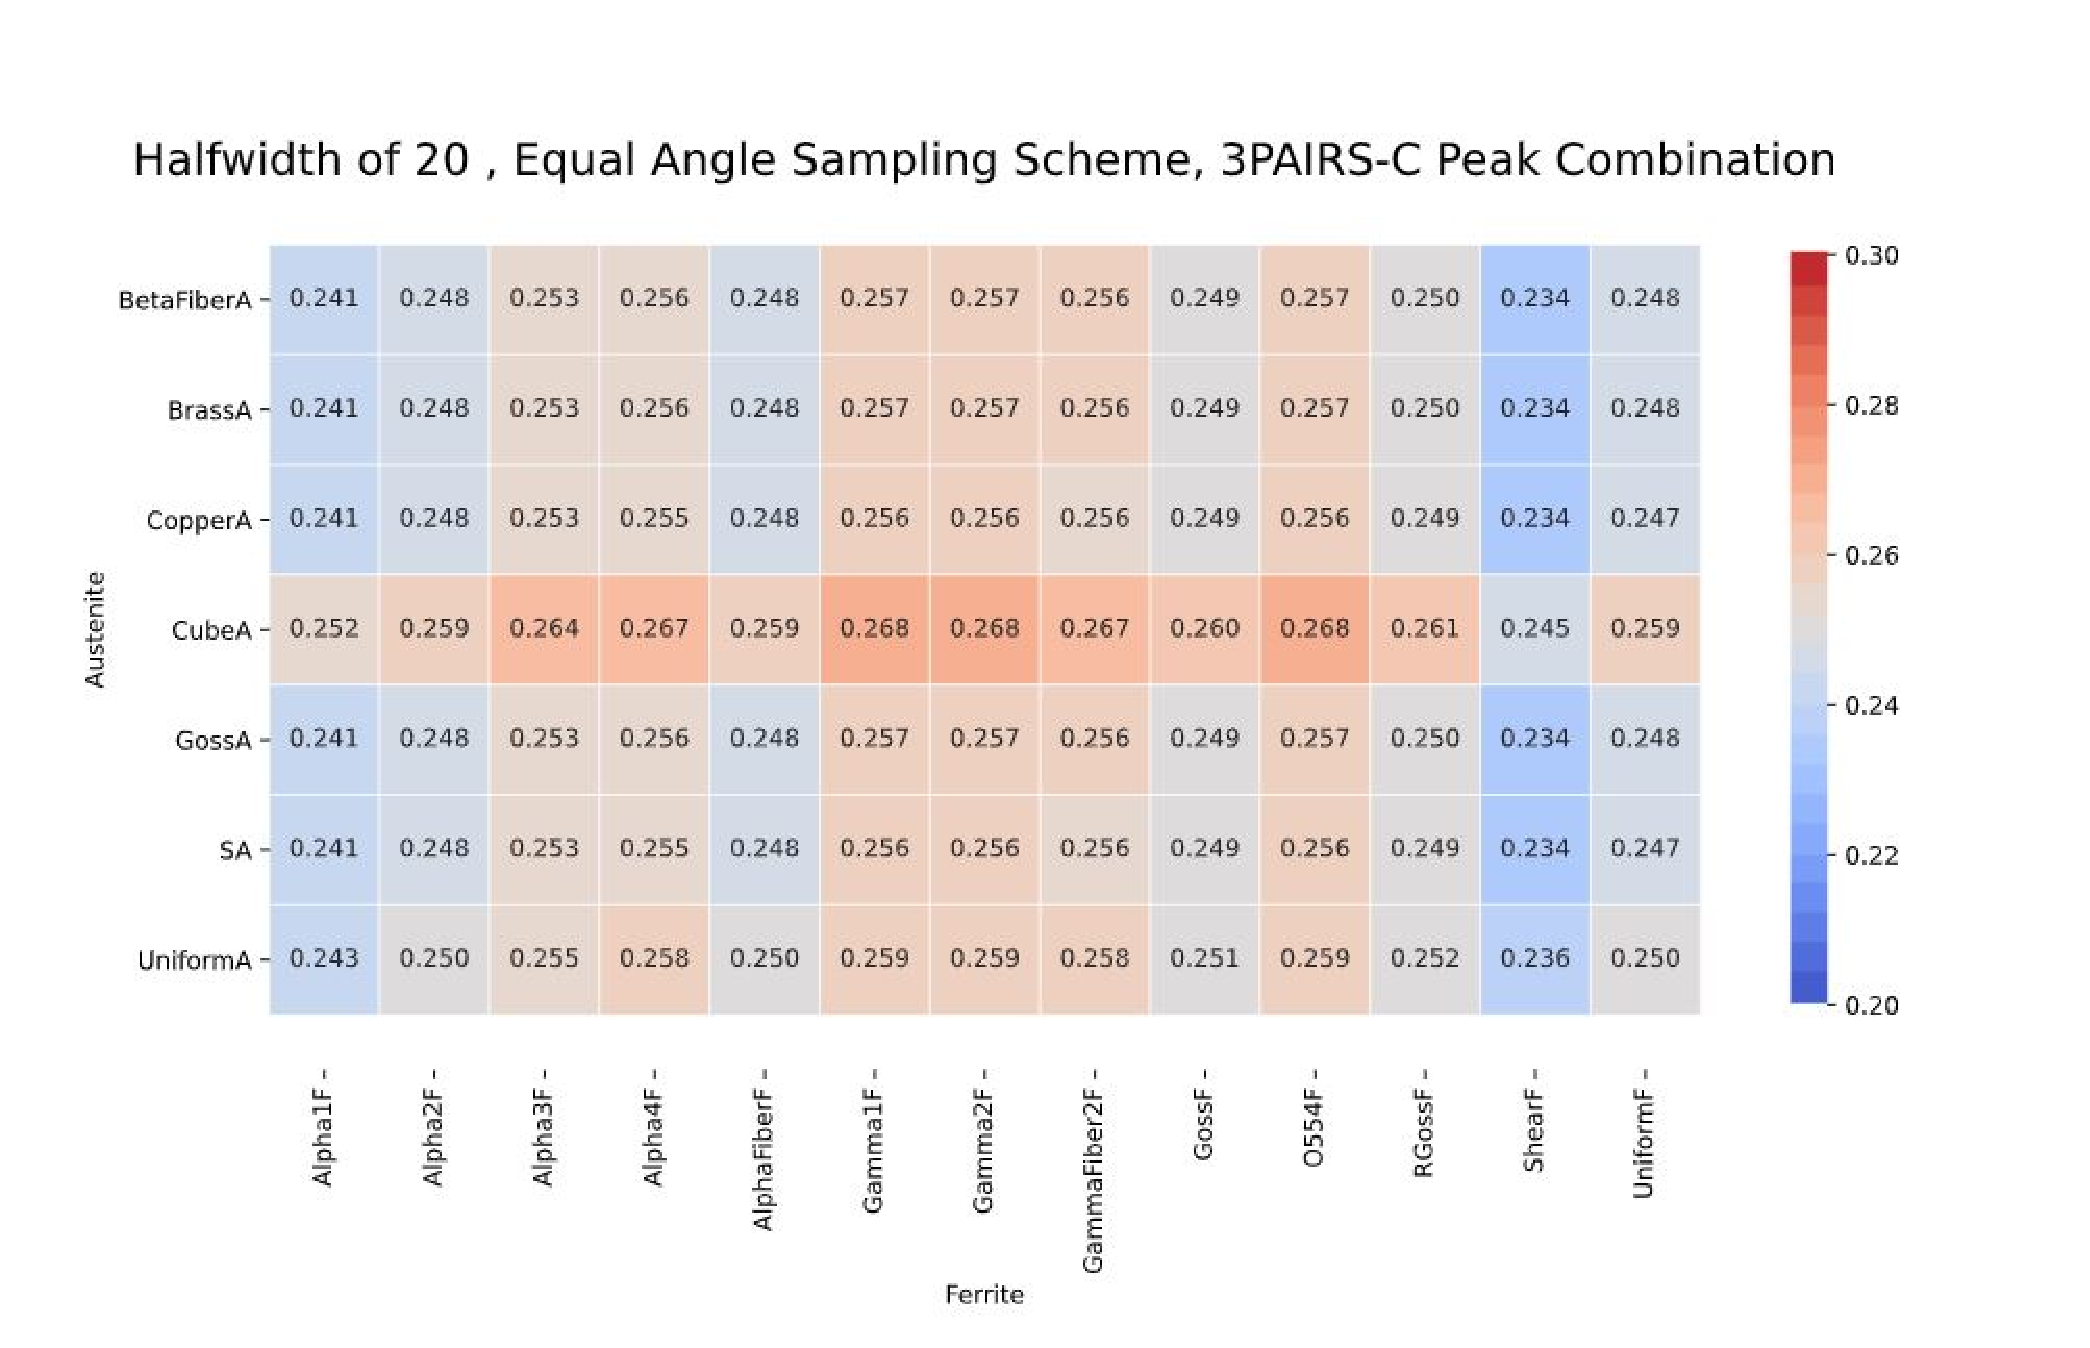
\includegraphics[width=10cm]{fig23}
    \caption{\label{tab1}The heatmap results for the Equal Angle scheme under fixed parameters. Overall, it struggles to effectively
    mititgate texture-induced measurement error.} 
    \end{figure}

As alluded to earlier, the uneven sampling distribution of this scheme, especially the oversampling along the ND axis, lends it to perform rather poorly 
in mitigating phase fraction measurement bias. With the exception of the Cube Austenite texture component, the remaining ferrite texture components 
seem to dominate in this measurement, considering how phase fraction values stay mostly consistent within columns for individual ferrite 
texture components. On the other hand, the Cube texture component seems to be the only austenite texture component that strongly impacts 
phase fraction measurement, mostly resulting in an overapproximation of the phase fraction value for this texture.

\subsubsection{CLR Grid Performance}
In contrast, the CLR grid performance is much more promising. As mentioned earlier, the
motivations for the CLR grid stem from distributing sampling points away 
from along the ND axis to more evenly cover the pole figure grid \cite{ref11}. To accomplish this,
the rotation increment was made a dynamic variable across changing tilts,
decreasing in magnitude as tilt increased. \textbf{Figure 24} provides the heatmap
figure results for this scheme conformed to the parameters alluded to in the
start of this section.

\begin{figure}[h]
    \centering
    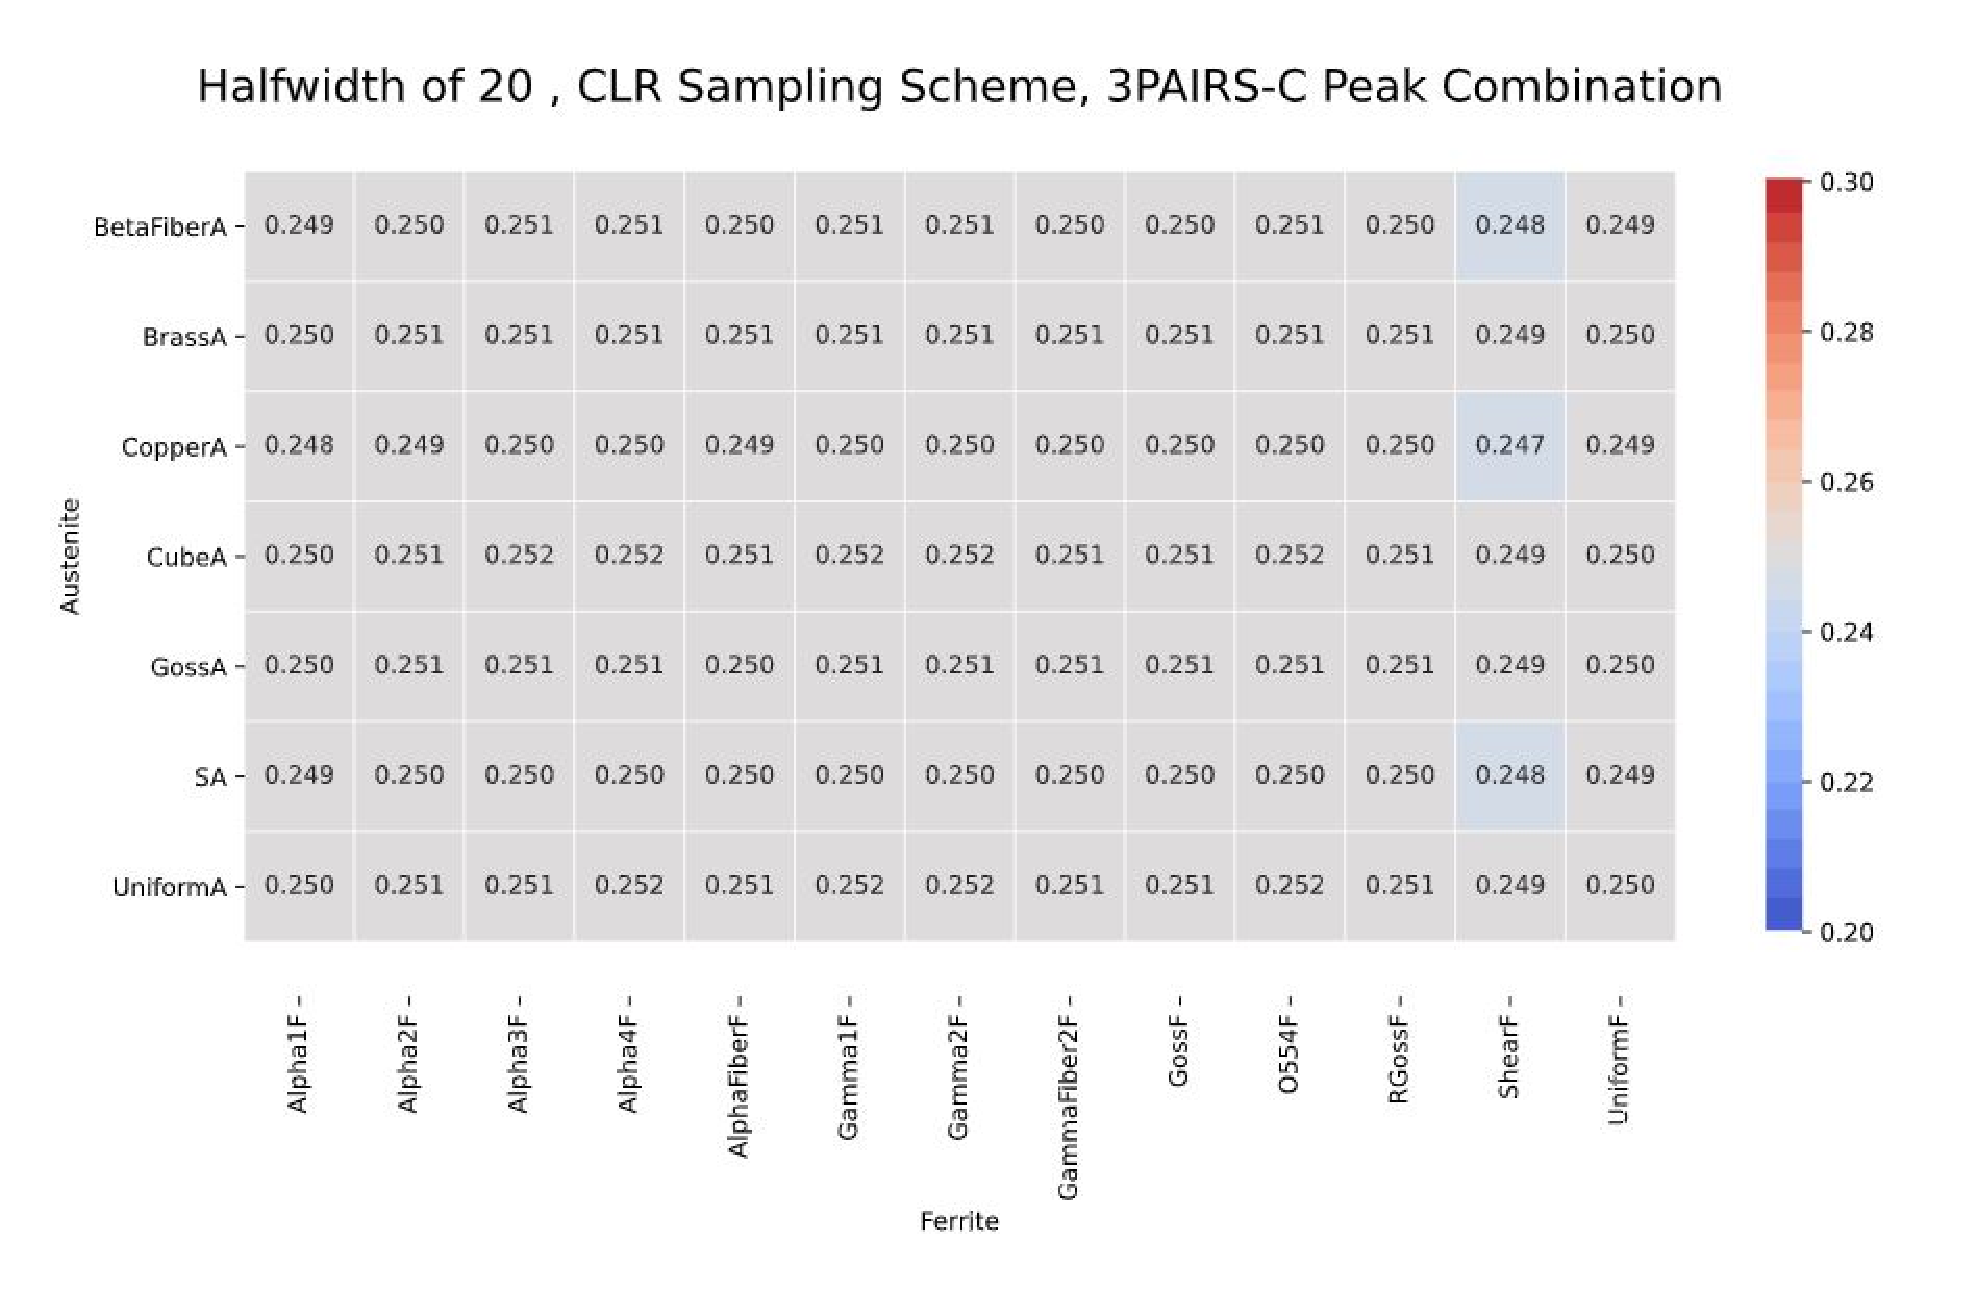
\includegraphics[width=10cm]{fig24}
    \caption{\label{tab1}The heatmap results for the CLR scheme under standard simulation parameters.} 
    \end{figure}

With nearly flawless performance, and considering that this scheme samples only
around 850 points, the CLR grid is overall a promising sampling scheme in combining
measurement accuracy with reduced sampling time. With the aforementioned parameters used,
there seem to be no systematic trends of problematic texture components impacting
phase fraction measurement bias. Analyzing the contour plot of this scheme back in
\textbf{Figure 16} confirms an overall even sampling of the grid, and consequently, a 
consistent and accurate measurement of phase fraction.

\subsubsection{Traditional Hex Scheme Performance}
The traditional hex scheme, as mentioned previously, has been known to provide the 
most promising combination of measurement accuracy across multiple variables
and reduced sampling time \cite{ref14}. A heatmap of its performance under the same parameters
outlined earlier in this section can be seen in \textbf{Figure 25}.

\begin{figure}[h]
    \centering
    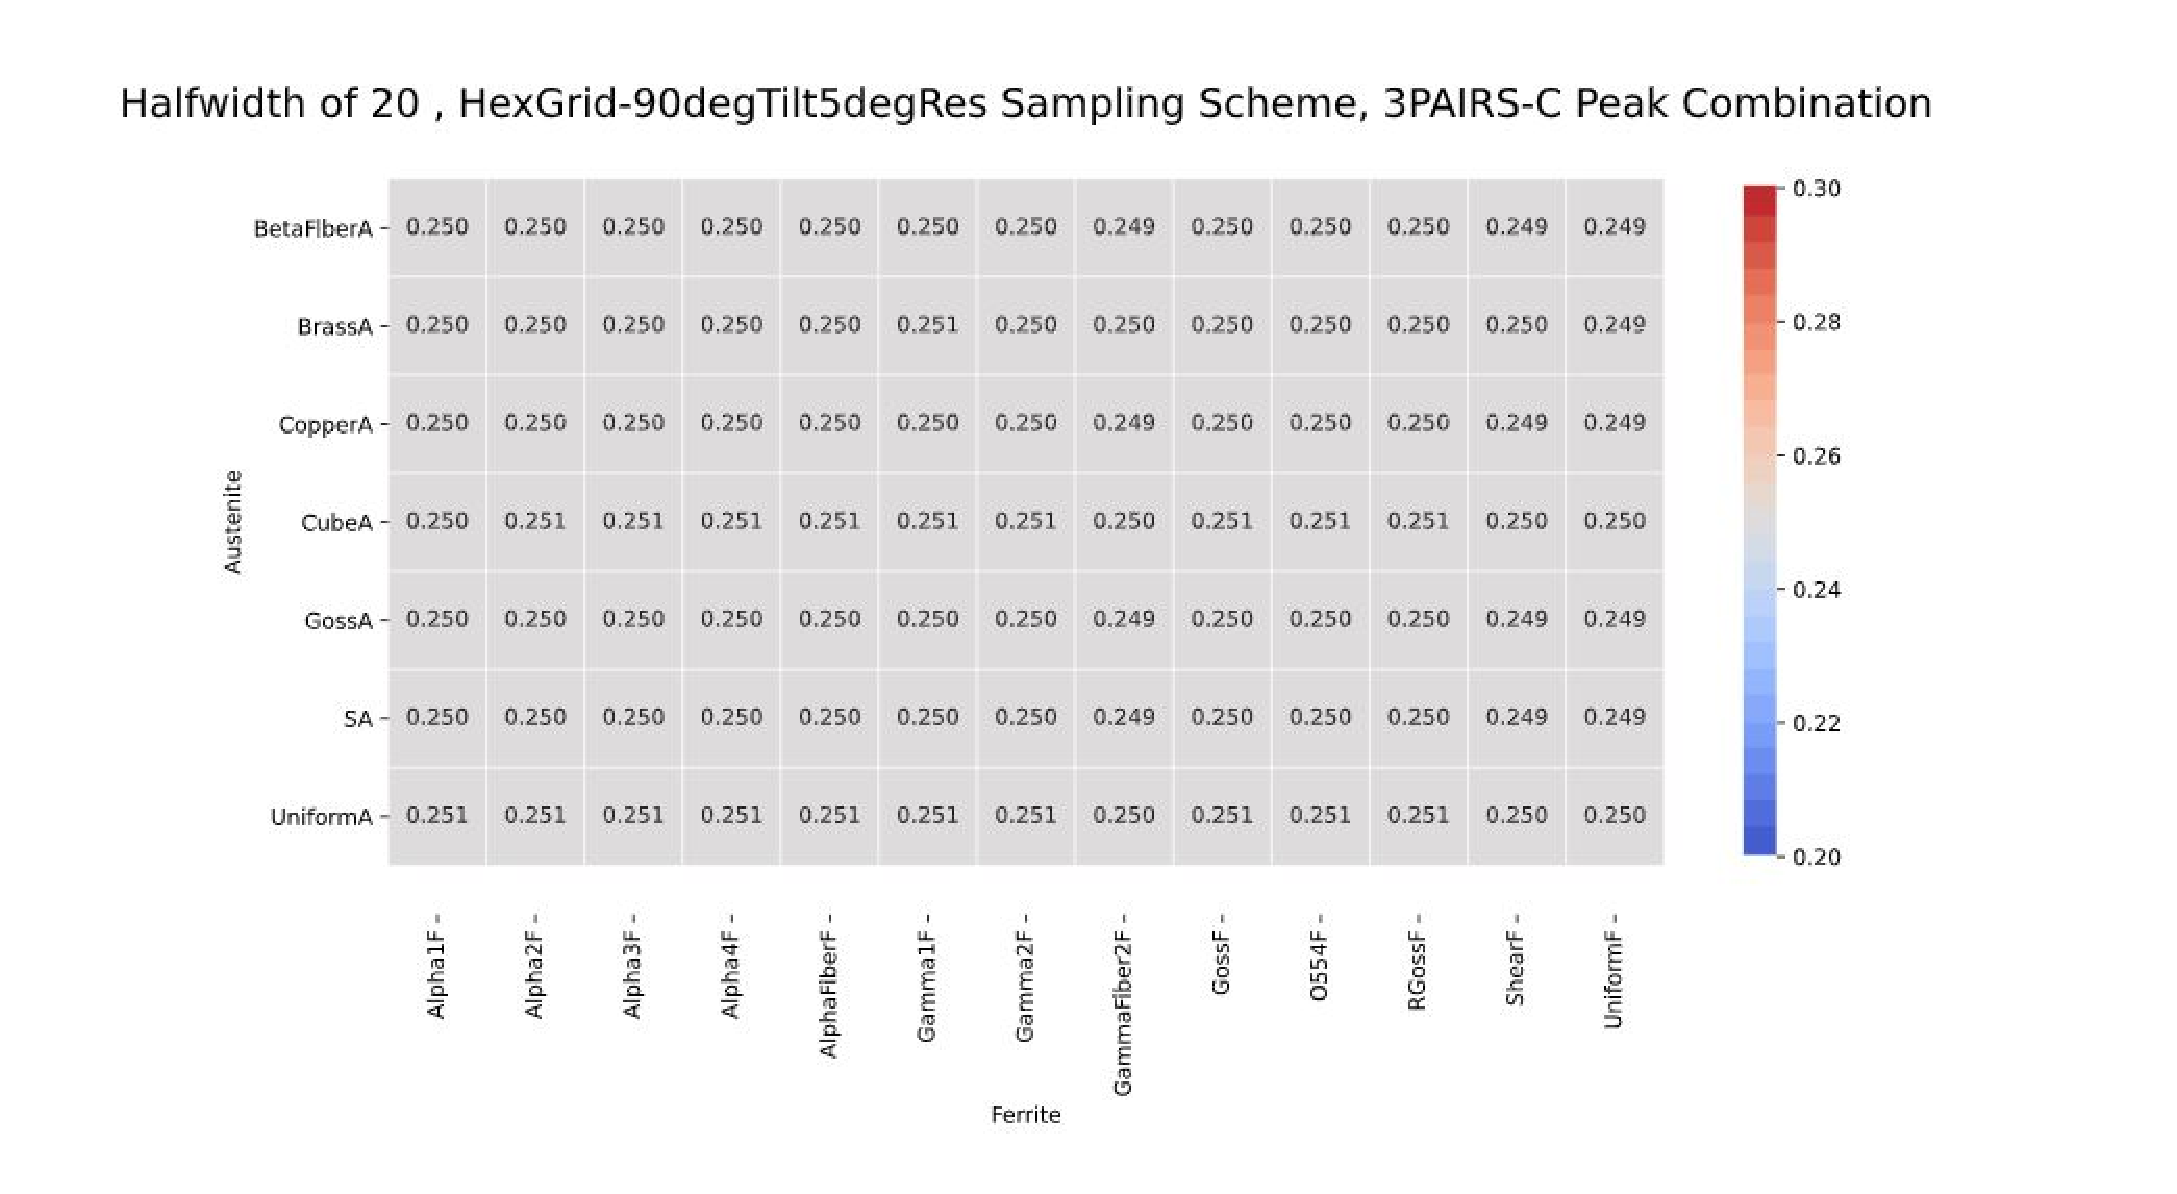
\includegraphics[width=10cm]{fig25}
    \caption{\label{tab1}The heatmap results for the traditional hex grid under standard simulation parameters.} 
    \end{figure}

Although slightly more accurate than the CLR grid under such parameters, 
the traditional hex scheme samples nearly 100 more points than the CLR grid.
With only slightly better performance, a logical comparison of the 
relative performance between both schemes can be made under the parameters used in
this simulation. 

\subsubsection{BT8\_Hex Scheme Performance}
The BT8\_Hex scheme attempts to recreate the same general pattern of the traditional hex scheme, but with roughly half the sampling points 
used. A heatmap of the results of this scheme can be seen in \textbf{Figure 26}.
\begin{figure}[h]
    \centering
    \includegraphics[width=9cm]{fig26}
    \caption{\label{tab1}The heatmap results for the BT8\_Hex grid under standard simulation parameters.} 
    \end{figure}

Although the BT8\_Hex scheme does not achieve the overall exact accuracy of the traditional hex scheme, or the CLR grid, there seem to be no
areas of consistent and significant phase fraction measurement error across all tested texture components. Furthermore, 
sampling nearly half as many points as the traditional hex scheme while achieving respectable measurement accuracy under the 
conditions elaborated above make this scheme an intriguing choice for phase fraction measurement purposes.

\subsubsection{Overall Comparison of Sampling Scheme Performance}
With the exception of the Equal Angle scheme, all other schemes tested under these standard conditions did not display
systematic measurement error in the presence of any given texture component. To evaluate scheme performance against each other, 
a \textbf{Violin Plot} was developed. Violin plots are similar to box and whisker plots in function, in that both techniques 
offer a basic summary of the distribution of quantitative data; however, violin plots can offer an added dimension of analysis on
how the data is distributed within the set, especially in scenarios where the distribution may have multiple peaks in data (bimodal, for example). Bulges in regions of the plot indicate areas of more frequent measurement, 
and represent such peaks in data, while thinner regions indiciate a sparse abundance of such data.
\textbf{Figure 27} provides a violin plot for all the schemes under the standard parameters discussed in this section.
\begin{figure}[h]
    \centering
    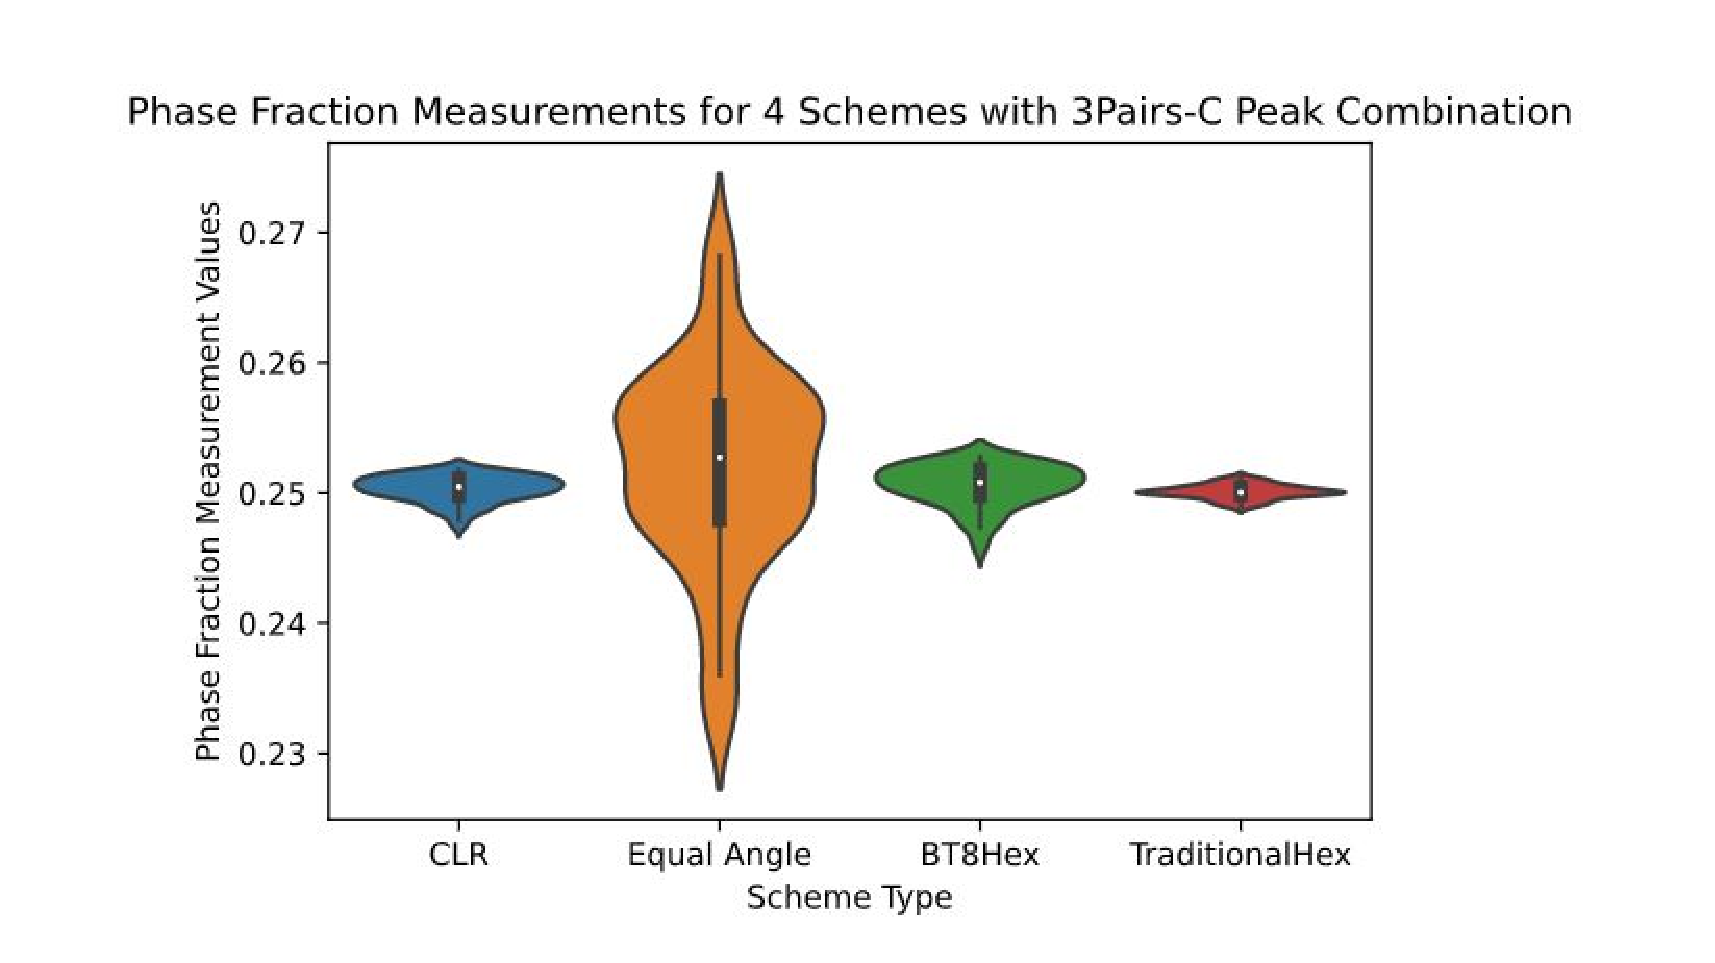
\includegraphics[width=10cm]{fig27}
    \caption{\label{tab1}A violin plot comparing scheme performance across standard simulation parameters.} 
    \end{figure}

The 2 biggest visual hints for evaluating scheme performance from a violin plot is the location of data bulges, and the "spread"
of such data. To elaborate, the ideal violin plot would have a single bulging region at a phase fraction value of 0.25, 
with the rest of the data located compactly along the bulge, with a limited spread. Analyzing the violin plot shown above, 
we can see that the traditional hex scheme best accomplishes both objectives, while the Equal Angle scheme occupies a much larger 
spread of data along with multiple regions of bulging in the plot. Both of these visual clues in the violin plot indicate a general inability for the Equal 
Angle scheme to consistently capture the theoretical 0.25 phase fraction value in the sample. Moving on, the BT8\_Hex scheme and the 
CLR Grid both seem to perform comparably well in removing measurement bias caused by texture, as jusitified by the compact nature of the 
violin plot and the single data bulge around the correct phase fraction value of 0.25. 

\subsection{Peak Combinations and Phase Fraction Measurement}
This section explores the second variable of interest in this project:
the impact of peak combinations on phase fraction measurement accuracy.
As a reminder, peaks in the XRD scan process are associated with crystal planes of a
desired material. In the calculation of phase fraction, certain peaks corresponding to the 
relevant material are integrated over the bounded area to solve for the phase fraction value. Although integrating 
across all possible peaks corresponding to a certain material would theoretically remove such measurement error,
the possibility of maintaining scheme accuracy across incorporating fewer peaks in the calcuation process is being explored 
in this project \cite{ref06}. On the flipside, incorporating much fewer peaks into the calculation process can theoretically introduce greater measurement
error as fewer crystal planes corresponding to a phase in the steel are used. However, especially in the presence of specific texture components aligned in certain
orientations, specific combinations of peaks can largely reduce the accuracy of phase fraction measurement; hence, the aforementioned
reasoning is not absolute by any means. 

For the most part, this following section will be broken down into subsections by scheme, discussing peak combinations and results of interest for
each scheme in this project. Special attention will be paid to peak combinations on the "extreme" end of the spectrum, such as the "1 Pair A" peak 
combination, which makes use of a single austenite and ferrite peak from the XRD scan graph output (refer to \textbf{Table 1} for more details on the exact peaks used).
Because including fewer peaks in the calculation process implies that fewer unique crystal planes corresponding to phases in a material are used, this exercise 
allows for problematic texture components 
to more readily manifest and contribute to significant measurement bias that can be observed via heatmaps.

As an aside, both the Equal Angle scheme and the traditional hex scheme do not have their own section of analysis for the effect of peak combinations on 
scheme performance. The behaviors of both these schemes, though diametrically opposite, are rather intuitive to understand. Due to its poor sampling of the pole figure, the Equal Angle 
scheme generates phase fractions as high as 0.3 
(in the presence of the Shear texture component) to as low as 0.19 (in the presence of the Cube texture component) for lower-order peak combinations (such as 1 and 2 pairs). On the other hand, the traditional hex scheme, again for 
intuitive reasons, maintains its remarkable performance with a nearly flawless capture of the desired 0.25 phase fraction value across all tested peak combinations.

Thus, the focus and 
emphasis of this section is on the 2 other schemes (CLR, BT8\_Hex) with performances that are not quite as intuitive to understand, making the following sections 
dedicated to exploring such results and offer some insight to explain the noticed behavior.

\subsubsection{Peak Combinations and CLR Grid Performance}
Although the CLR grid does not have any regions of poor sampling in particular when analyzing the scheme pole figure, there are certain 
texture components which can systematically induce some measurement error for this scheme. To clarify, such measurement bias is not as extreme 
as the error observed for the Equal Angle scheme, but is still an area of improvement for this scheme. \textbf{Figure 28} provides a heatmap for this scheme using
the 1 Pair A peak combination, which induced the most measurement error of any peak combination.
\begin{figure}[h]
    \centering
    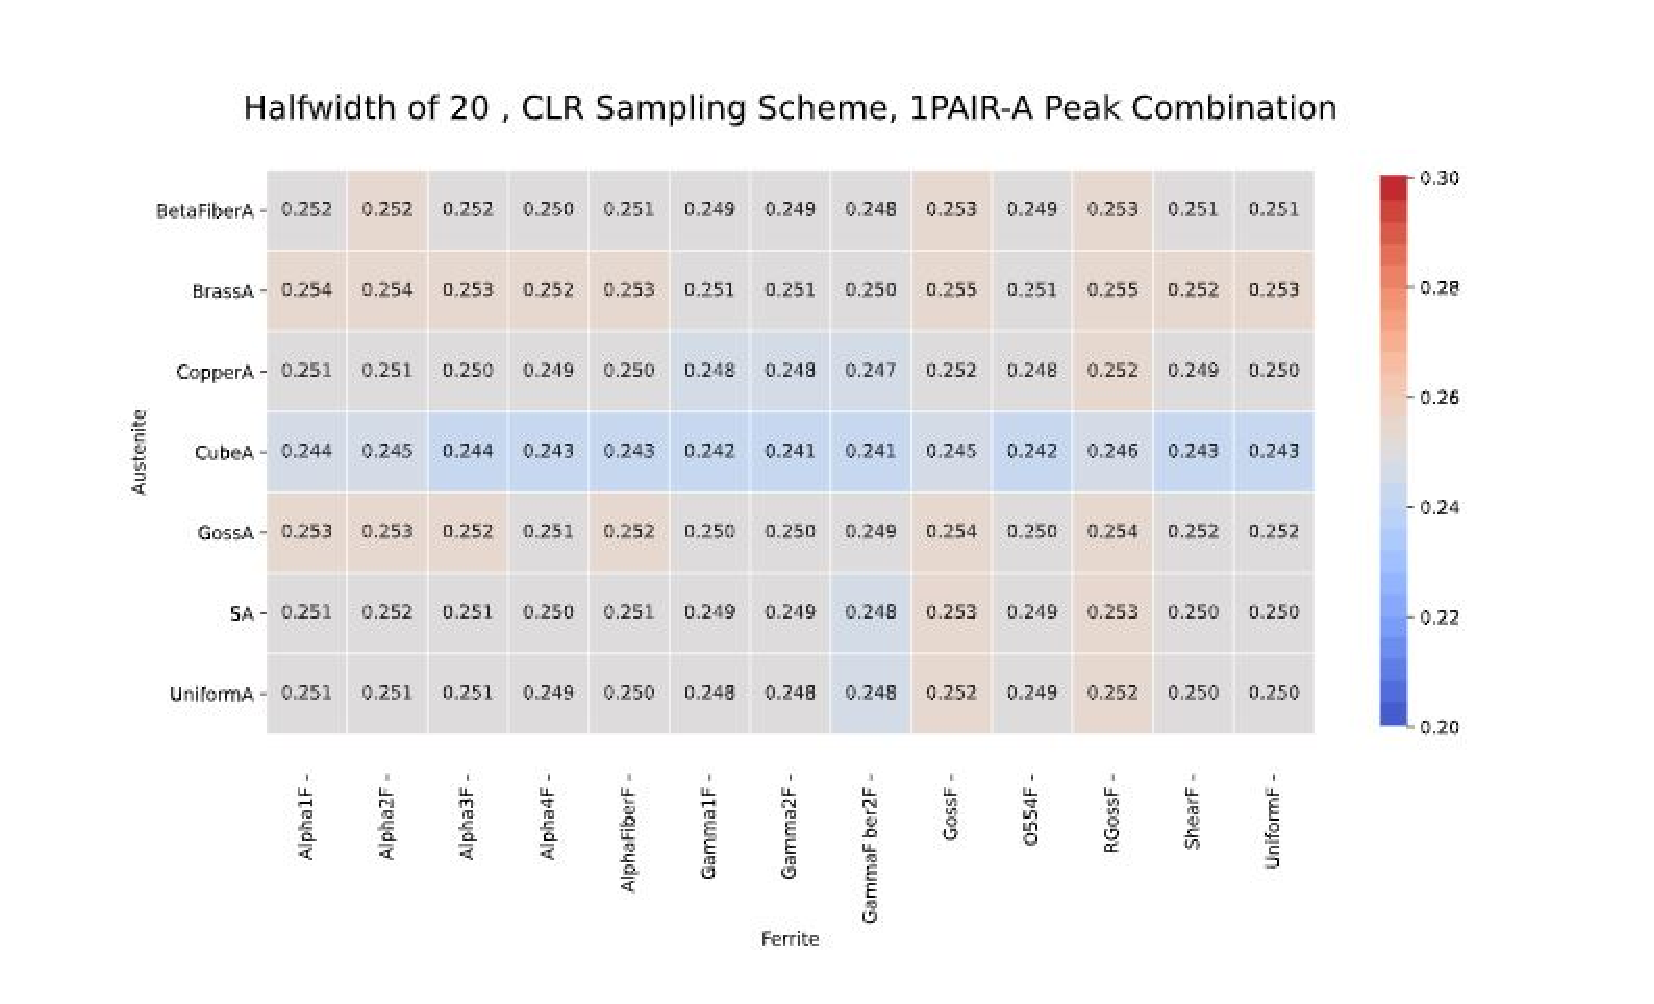
\includegraphics[width=10cm]{fig28}
    \caption{\label{tab1}The heatmap results for the CLR grid under the 1 Pair peak combination.} 
    \end{figure}

The most significant and impactful texture component displayed above is the Cube texture component, a simplification of which can be visualized in \textbf{Figure 29}.
\begin{figure}[h]
    \centering
    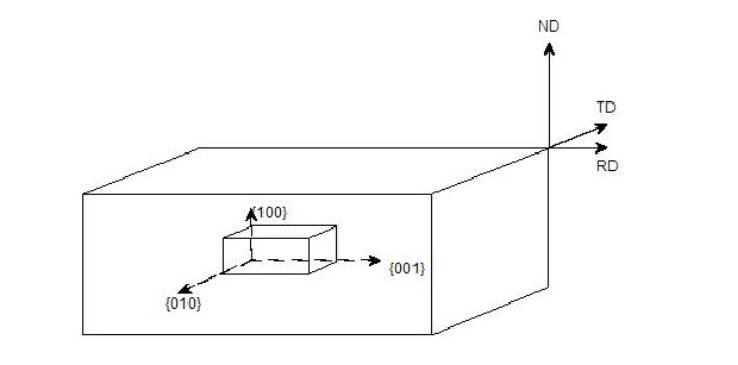
\includegraphics[width=10cm]{fig29}
    \caption{\label{tab1}An intuitive visualization of the Cube texture component. Adapted from \cite{ref08}. } 
    \end{figure}

Considering how phase fraction measurements are consistently underestimated for the Cube texture component, it is clear that this texture component
dominates phase fraction measurement irrespective of other textures. 

To understand why the Cube texture component under the 1 Pair A peak combination impacts the ability for the CLR grid to accurately 
capture phase fraction values, we can look at the contour plot pole figure for the Cube texture component at the orientations included under 
the 1 Pair peak combination. \textbf{Figure 30} provides the pole figure plot for the Cube texture under the (111) orientation plane, which is the retained 
austenite plane used in this peak combination.
\begin{figure}[h]
    \centering
    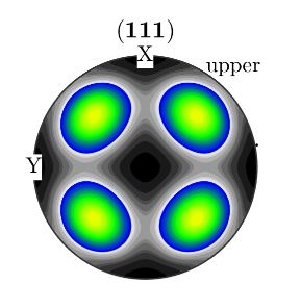
\includegraphics[width=8.5cm]{fig30}
    \caption{\label{tab1}A contour plot of the Cube texture component using the (111) orientation plane.} 
    \end{figure}

This, analyzed in conjunction with the oversampling contour plot for the CLR grid, as shown back in \textbf{Figure 16}, can provide some reasoning for why the Cube texture 
appears more problematically under this scheme.

Judging the contour plot for this scheme, it is clear that regions in between the center and perimeter of the plot are not as evenly sampled as the perimeter of the 
sampling scheme pole figure. This can be inferred by the fact that such regions are shaded grey (uneven sampling), while the perimeter regions are marked blue (even sampling).
Consequently, the Cube texture component's contour plot for the (111) plane shows regions of uneven intensities in similar regions (marked light green and yellow), which would intuitively cause 
phase fraction measurements to be biased. 

It is important to keep in mind, however, that the factor of sampling (sampling multiples) experienced in this region of interest for this scheme is not major (it is a little bit under 1). As a result of this,
the phase fraction values do not deviate incredibly from the target value of 0.25. Although the Cube texture component appeared most consistently problematic for this scheme, and reasons 
for such behavior were offered, the CLR grid overall still does a respectable job in mitigating phase fraction measurement bias overall as evidenced by the heatmap in this section (\textbf{Figure 28}), which
consists of measurements in the range of [0.241, 0.255]. Other tested peak combinations improved on this measurement range with increasing peaks used in the calculation, so only the 1 Pair peak combination was explicitly analyzed in this section 
(as it offered the most statistically significant deviations from the expected phase fraction as compared to other peak combinations).

\subsubsection{Peak Combinations and BT8\_Hex Grid Performance}
By far, the most noticeable feature in the implementation of the BT8\_Hex grid is the oversampling across the perimeter regions of the pole figure. Therefore, following a similar reasoning used above, we can make connections between oversampling plots for the 
sampling scheme and the corresponding texture component pole figures. To begin, \textbf{Figure 31} provides the heatmap summarizing the simulation 
results of this scheme using the 1 Pair A peak combination once again (as this peak combination provided the most measurement error of any peak combination).
\begin{figure}[h]
    \centering
    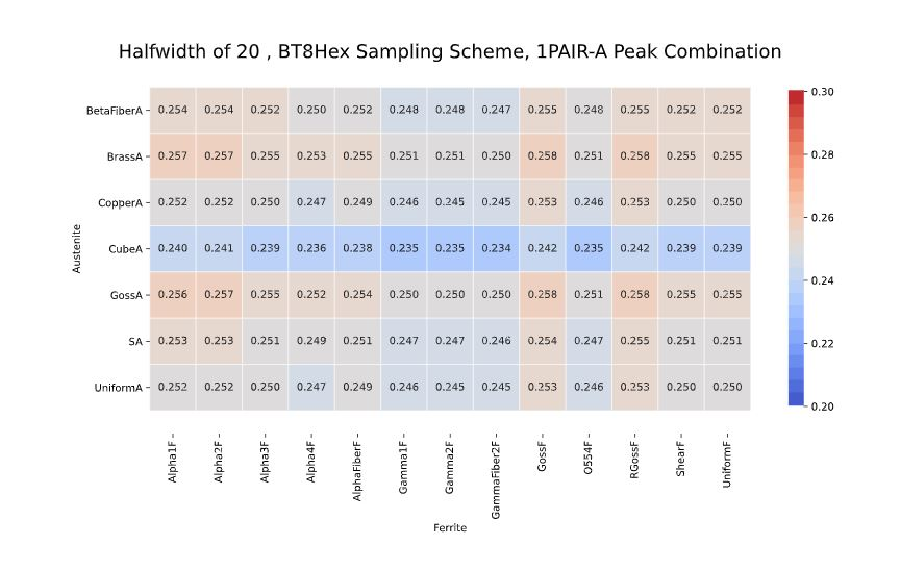
\includegraphics[width=10cm]{fig31}
    \caption{\label{tab1}The heatmap results of the BT8\_Hex grid under the 1 Pair A peak combination.} 
    \end{figure}

Once again, the Cube texture component dominates the simulation and results in an underestimation of phase fraction value; however, the RGoss ferrite texture and the Brass austenite texture also induce measurement bias by an overestimation of phase fractions. Understanding the texture component pole figures (the Cube texture can be seen back in \textbf{Figure 31}) 
for each of these texture components, and the oversampling contour plot for the BT8\_Hex scheme (as shown back in \textbf{Figure 21}) can provide some intuitive 
reasoning for such phenomena.

Let us begin with analysis of the Cube texture, which we have had previous exposure to in the past section. The plot for this texture component (refer back to \textbf{Figure 30}) shows 
extremely low intensities along the perimeter edges of the plot, which coincides with the uneven sampling of the BT8\_Hex along such peripheral regions of the 
contour plot. This provides a simple reason for the underestimation of phase fraction value that the Cube texture causes for this scheme and peak combination.

Next, the Brass texture, which, like the Cube texture, is also a texture appearing in the retained austenite phase, can be explored. Because this texture appears in the retained austenite phase, the (111) plane orientation pole 
figure will be used to study this texture, as
we did similarly for the Cube texture. This contour plot pole figure for this 
texture component can be seen in \textbf{Figure 32}.
\begin{figure}[h]
    \centering
    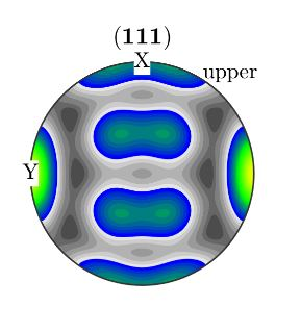
\includegraphics[width=8.5cm]{fig32}
    \caption{\label{tab1}A contour plot of the Brass texture component using the (111) orientation plane.} 
    \end{figure}

The most significant regions of uneven diffracted intensities appear towards the left and right edges of this figure, which are marked in green on either side.
These regions also correspond with the outer regions of the BT8\_Hex grid which are unevenly sampled, inducing some level of measurement bias and 
providing reasonable explanation for why this texture component appears a bit more problematically for this BT8\_Hex scheme.

Finally, the RGoss texture will be explored. This texture appears in the ferrite phase of the steel, so a different orientation must be 
used for studying this texture component's contour pole figure. Specifically, the (110) orientation of this texture component's pole figure will be 
analyzed, as this orientation is the single ferrite peak used for the 1 Pair A peak combination. The plot for this texture component constrained by the details mentioned 
above can be seen in \textbf{Figure 33}.
\begin{figure}[h]
    \centering
    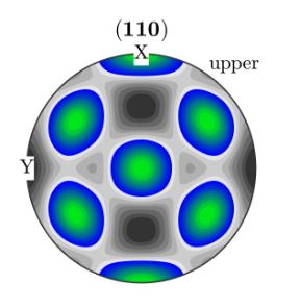
\includegraphics[width=8.5cm]{fig33}
    \caption{\label{tab1}A contour plot of the RGoss texture component using the (110) orientation plane.} 
    \end{figure}

For this texture component, along with stronger intensities towards the middle regions of the plot, holds weaker diffraction intensities along left and 
right edges of the pole figure and stronger measured intensities at the "North" and "South" poles of the plot. Along with oversampling along the edges of the plot, 
the BT8\_Hex scheme also holds significant regions of gray (slightly uneven sampling) towards the middle of the plot (see \textbf{Figure 21}), similar to the CLR grid. The 
combination of these 3 factors (weaker intensities on the left and right edges of plot, stronger intensities towards the middle of the plot and at the North and South poles) 
contribute to why the BT8\_Hex scheme struggles a bit more than usual with the RGoss texture component.

Once again, the magnitude of measurement bias from all these texture components is not incredibly grave: holistically, the BT8\_Hex scheme
performs admirably in mitigating egregious phase fraction measurement error, recording measurements in the range of [0.234, 0.258]. However,
there are certain texture components (such as Cube, Brass, and RGoss) that induce more systematic measurement bias than other textures. Once again, 
other peak combinations were also explored but not explicitly analyzed in this project, as intuitively, phase fraction measurement improved 
as more peaks were incorporated into the calculation process. Similar to the CLR analysis in the previous section, the 1 Pair A peak combination provided the most statistically significant
measurement error compared to other tested peak combinations, which is why it was the only combination explicitly analyzed in this section.

\subsubsection{Overall Comparison and Summary of Peak Combinations and Scheme Performance}
Though not absolute, some general trends can be observed as we vary the peak combinations used in calculation to measure the ensuing phase fraction 
values. For lower-order peak combinations (such as 1-2 Pair), larger measurement bias was observed across all schemes, as fewer peaks 
corresponding to the retained austenite phase were incorporated into the calculation. For the Equal Angle scheme 
and the traditional hex grid, the results were fairly intuitive: due to the extreme uneven sampling of the Equal Angle grid, 
measurement error was largely exacerbated, with values in the range of [0.19, 0.30]. On the other hand, the traditional hex scheme maintained 
its exceptional ability to account for all texture-induced bias, recording consistent measurements in the range of [0.250, 0.252].

The CLR grid and BT8\_Hex scheme, however, provided some interesting results that may not be as intuitive to understand at first glance.
Both schemes struggled most with the Cube texture component, with the Brass and RGoss textures addtionally appearing as problematic for the 
BT8\_Hex grid. This can be attributed to the oversampling experienced by the BT8\_Hex grid, especially towards the perimeter of the 
contour plot. Although the CLR grid doesn’t include such regions of uneven sampling, the middle sections of the plot hold regions of very slight 
undersampling (shown as gray in the plot), which can explain why this scheme struggles a bit with the Cube texture. Ultimately, the magnitude of 
measurement error for both schemes is rather marginal; however, the systematic error measured in the presence of certain textures was explored and 
attributed to the uneven nature of sampling in some regions of both these schemes.

A summary of such measurements (using the 1 Pair A peak combination) can be captured in the Violin plot provided in \textbf{Figure 34}.
\begin{figure}[h]
    \centering
    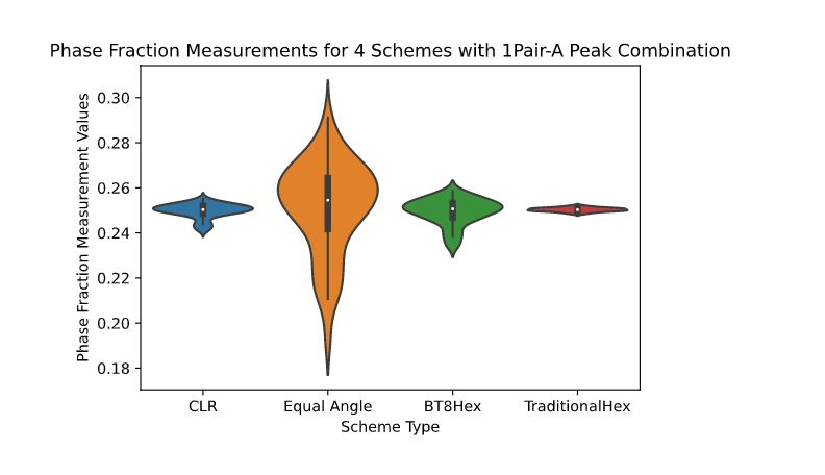
\includegraphics[width=10cm]{fig34}
    \caption{\label{tab1}A violin plot comparing scheme performance under the 1 Pair A peak combination.} 
    \end{figure}

\section{Concluding Thoughts and Ideas for Future Work}
This section will provide an overview of the results discovered throughout this project, while looking ahead to future areas of research that
stem from this project experience.
\subsection{Project Summary}
Over the 12 week research period of this project, 4 novel schemes were computationally developed and tested by simulation for their ability to mitigate 
phase fraction measurement bias: the Equal Angle scheme, the CLR Grid, the Traditional Hex scheme, and the BT8\_Hex grid. Furthermore, 
the effect of peak combinations on phase fraction calculation for these 4 schemes was also investigated. This report provided an in-depth review of background topics 
necessary to appreciate this research, followed by a summary and analysis of the project findings. Succintly, it was determined that, under 
standard simulation conditions, the traditional hex, CLR grid, and BT8\_Hex grid all were able to effectively mititgate phase fraction measurement bias, 
with all 3 schemes recording measurements within the range of [0.247, 0.253]. On the other hand, the Equal Angle scheme, as evidenced by the 
uneven nature of its sampling, fails to consistently record accurate measurements of phase fraction, with its measurement values occupying the 
range of approximately [0.23, 0.27]. In the analysis of peak combinations and phase fraction measurement, a general relationship between the 
number of peaks incorporated and the effectiveness of phase fraction measurement could be made (though this statement is not absolute). To elaborate, 
the 1-Pair peak combination resulted in poor measurements for the Equal Angle scheme, in the range of [0.19, 0.30]. On the other hand, the CLR grid and BT8\_Hex scheme held measurements in the 
ranges of [0.240, 0.255] and [0.23, 0.26], respectively. Although such ranges remain respectably about the expected phase fraction of 0.25, 
there are certain texture components, such as the Cube texture, which induce systematic underestimations of phase fraction measurement. The 
traditional hex grid, as expected, maintains remarkable measurement accuracy across all peak combinations, and there seem to be no texture components that cause
systematic measurement bias for this scheme. However, the traditional hex scheme samples nearly 950 points, while the CLR grid samples nearly 850 points 
and the BT8\_Hex samples nearly 470 points; therefore, under most simulation conditions, a reasonable comparison between these 3 schemes can be made, considering both 
scheme performance and the feasibility/reduced sampling time that accompanies both the CLR grid and BT8\_Hex scheme.

\subsection{Plans for Future Work}
Of course, there were some obvious limitations on the topics that could have been covered under the 
field of improving the retained austenite phase fraction measurement process. Ideas for immediate future work include the implementation and
testing of new schemes (such as the Gaussian Quadrature and Rotated Ring Schemes) for their ability to account for phase fraction measurement 
bias. Another point of further exploration could be the improvement of current scheme models: for example, addressing the oversampling along 
the outer ring of the BT8\_Hex scheme, or verifying the sampling coordinates of the CLR grid scheme (since a bit of rounding was used in the implementation of 
that scheme). A final area of interest is developing novel methods to avoid problematic texture components (as defined by heatmaps) by selectively scanning 
specific areas of the sample \cite{ref14}. This research would likely deal with the preparation of sampling media to ensure accurate results more than the 
process of X-ray diffraction itself.

Further down the line, the most promising combinations of sampling schemes and peak combinations will be tested by 
experimentation in labs 
to see if the promising results suggested via simulation can be consistently upheld in the actual scanning process \cite{ref14}. The hope for these 
findings down the line is to ultimately generate new standards of XRD sampling procedures that accurately and effectively 
conduct phase fraction measurements for users and producers of steel alike.



\section{Acknowledgements}
I would like to thank several people who have helped me throughout both the SRP and the report-writing process. Firstly, to my teachers 
throughout the years, for helping me develop an affinity for multiple subjects such as mathematics, science, and literature, all which 
came to good use in the production of this paper. Next to my mentors, both faculty and on-site, for their continued guidance
and feedback throughout this entire process to ensure this report remained streamlined and persuasive. Lastly, to ASPPRC and the Department of 
Metallurgical and Materials Engineering at the Colorado School of Mines, for the opportunity to work on such a project and for providing me
with the resources and support necessary to independently execute this SRP.

\bibliography{IEEEabrv,icdp2009}


\end{document}














